\documentclass[twoside]{book}

% Packages required by doxygen
\usepackage{calc}
\usepackage{doxygen}
\usepackage{graphicx}
\usepackage[utf8]{inputenc}
\usepackage{makeidx}
\usepackage{multicol}
\usepackage{multirow}
\usepackage{textcomp}
\usepackage[table]{xcolor}

% Font selection
\usepackage[T1]{fontenc}
\usepackage{mathptmx}
\usepackage[scaled=.90]{helvet}
\usepackage{courier}
\usepackage{amssymb}
\usepackage{sectsty}
\renewcommand{\familydefault}{\sfdefault}
\allsectionsfont{%
  \fontseries{bc}\selectfont%
  \color{darkgray}%
}
\renewcommand{\DoxyLabelFont}{%
  \fontseries{bc}\selectfont%
  \color{darkgray}%
}

% Page & text layout
\usepackage{geometry}
\geometry{%
  a4paper,%
  top=2.5cm,%
  bottom=2.5cm,%
  left=2.5cm,%
  right=2.5cm%
}
\tolerance=750
\hfuzz=15pt
\hbadness=750
\setlength{\emergencystretch}{15pt}
\setlength{\parindent}{0cm}
\setlength{\parskip}{0.2cm}
\makeatletter
\renewcommand{\paragraph}{%
  \@startsection{paragraph}{4}{0ex}{-1.0ex}{1.0ex}{%
    \normalfont\normalsize\bfseries\SS@parafont%
  }%
}
\renewcommand{\subparagraph}{%
  \@startsection{subparagraph}{5}{0ex}{-1.0ex}{1.0ex}{%
    \normalfont\normalsize\bfseries\SS@subparafont%
  }%
}
\makeatother

% Headers & footers
\usepackage{fancyhdr}
\pagestyle{fancyplain}
\fancyhead[LE]{\fancyplain{}{\bfseries\thepage}}
\fancyhead[CE]{\fancyplain{}{}}
\fancyhead[RE]{\fancyplain{}{\bfseries\leftmark}}
\fancyhead[LO]{\fancyplain{}{\bfseries\rightmark}}
\fancyhead[CO]{\fancyplain{}{}}
\fancyhead[RO]{\fancyplain{}{\bfseries\thepage}}
\fancyfoot[LE]{\fancyplain{}{}}
\fancyfoot[CE]{\fancyplain{}{}}
\fancyfoot[RE]{\fancyplain{}{\bfseries\scriptsize Generated on Mon Dec 7 2015 14\-:38\-:25 for R\-A\-P\-P Platform Tests -\/ Audio Processing by Doxygen }}
\fancyfoot[LO]{\fancyplain{}{\bfseries\scriptsize Generated on Mon Dec 7 2015 14\-:38\-:25 for R\-A\-P\-P Platform Tests -\/ Audio Processing by Doxygen }}
\fancyfoot[CO]{\fancyplain{}{}}
\fancyfoot[RO]{\fancyplain{}{}}
\renewcommand{\footrulewidth}{0.4pt}
\renewcommand{\chaptermark}[1]{%
  \markboth{#1}{}%
}
\renewcommand{\sectionmark}[1]{%
  \markright{\thesection\ #1}%
}

% Indices & bibliography
\usepackage{natbib}
\usepackage[titles]{tocloft}
\setcounter{tocdepth}{3}
\setcounter{secnumdepth}{5}
\makeindex

% Hyperlinks (required, but should be loaded last)
\usepackage{ifpdf}
\ifpdf
  \usepackage[pdftex,pagebackref=true]{hyperref}
\else
  \usepackage[ps2pdf,pagebackref=true]{hyperref}
\fi
\hypersetup{%
  colorlinks=true,%
  linkcolor=blue,%
  citecolor=blue,%
  unicode%
}

% Custom commands
\newcommand{\clearemptydoublepage}{%
  \newpage{\pagestyle{empty}\cleardoublepage}%
}


%===== C O N T E N T S =====

\begin{document}

% Titlepage & ToC
\hypersetup{pageanchor=false}
\pagenumbering{roman}
\begin{titlepage}
\vspace*{7cm}
\begin{center}%
{\Large R\-A\-P\-P Platform Tests -\/ Audio Processing \\[1ex]\large 0.\-5.\-5 }\\
\vspace*{1cm}
{\large Generated by Doxygen 1.8.6}\\
\vspace*{0.5cm}
{\small Mon Dec 7 2015 14:38:25}\\
\end{center}
\end{titlepage}
\clearemptydoublepage
\tableofcontents
\clearemptydoublepage
\pagenumbering{arabic}
\hypersetup{pageanchor=true}

%--- Begin generated contents ---
\chapter{Namespace Index}
\section{Namespace List}
Here is a list of all namespaces with brief descriptions\-:\begin{DoxyCompactList}
\item\contentsline{section}{\hyperlink{namespacecognitive__exercise}{cognitive\-\_\-exercise} }{\pageref{namespacecognitive__exercise}}{}
\item\contentsline{section}{\hyperlink{namespacecognitive__exercise__main}{cognitive\-\_\-exercise\-\_\-main} }{\pageref{namespacecognitive__exercise__main}}{}
\item\contentsline{section}{\hyperlink{namespacemysql__wrapper}{mysql\-\_\-wrapper} }{\pageref{namespacemysql__wrapper}}{}
\item\contentsline{section}{\hyperlink{namespacemysql__wrapper__main}{mysql\-\_\-wrapper\-\_\-main} }{\pageref{namespacemysql__wrapper__main}}{}
\item\contentsline{section}{\hyperlink{namespacerapp__audio__processing}{rapp\-\_\-audio\-\_\-processing} }{\pageref{namespacerapp__audio__processing}}{}
\item\contentsline{section}{\hyperlink{namespacerapp__audio__processing_1_1rapp__audio__processing}{rapp\-\_\-audio\-\_\-processing.\-rapp\-\_\-audio\-\_\-processing} }{\pageref{namespacerapp__audio__processing_1_1rapp__audio__processing}}{}
\item\contentsline{section}{\hyperlink{namespacerapp__audio__processing_1_1rapp__detect__silence}{rapp\-\_\-audio\-\_\-processing.\-rapp\-\_\-detect\-\_\-silence} }{\pageref{namespacerapp__audio__processing_1_1rapp__detect__silence}}{}
\item\contentsline{section}{\hyperlink{namespacerapp__audio__processing_1_1rapp__energy__denoise}{rapp\-\_\-audio\-\_\-processing.\-rapp\-\_\-energy\-\_\-denoise} }{\pageref{namespacerapp__audio__processing_1_1rapp__energy__denoise}}{}
\item\contentsline{section}{\hyperlink{namespacerapp__audio__processing_1_1rapp__set__noise__profile}{rapp\-\_\-audio\-\_\-processing.\-rapp\-\_\-set\-\_\-noise\-\_\-profile} }{\pageref{namespacerapp__audio__processing_1_1rapp__set__noise__profile}}{}
\item\contentsline{section}{\hyperlink{namespacerapp__audio__processing_1_1rapp__sox__denoise}{rapp\-\_\-audio\-\_\-processing.\-rapp\-\_\-sox\-\_\-denoise} }{\pageref{namespacerapp__audio__processing_1_1rapp__sox__denoise}}{}
\item\contentsline{section}{\hyperlink{namespacerapp__audio__processing_1_1rapp__transform__audio}{rapp\-\_\-audio\-\_\-processing.\-rapp\-\_\-transform\-\_\-audio} }{\pageref{namespacerapp__audio__processing_1_1rapp__transform__audio}}{}
\item\contentsline{section}{\hyperlink{namespacerapp__audio__processing_1_1rapp__utilities}{rapp\-\_\-audio\-\_\-processing.\-rapp\-\_\-utilities} }{\pageref{namespacerapp__audio__processing_1_1rapp__utilities}}{}
\item\contentsline{section}{\hyperlink{namespacerapp__exceptions}{rapp\-\_\-exceptions} }{\pageref{namespacerapp__exceptions}}{}
\item\contentsline{section}{\hyperlink{namespacerapp__speech__detection__sphinx4}{rapp\-\_\-speech\-\_\-detection\-\_\-sphinx4} }{\pageref{namespacerapp__speech__detection__sphinx4}}{}
\item\contentsline{section}{\hyperlink{namespacerapp__speech__detection__sphinx4_1_1english__support}{rapp\-\_\-speech\-\_\-detection\-\_\-sphinx4.\-english\-\_\-support} }{\pageref{namespacerapp__speech__detection__sphinx4_1_1english__support}}{}
\item\contentsline{section}{\hyperlink{namespacerapp__speech__detection__sphinx4_1_1global__parameters}{rapp\-\_\-speech\-\_\-detection\-\_\-sphinx4.\-global\-\_\-parameters} }{\pageref{namespacerapp__speech__detection__sphinx4_1_1global__parameters}}{}
\item\contentsline{section}{\hyperlink{namespacerapp__speech__detection__sphinx4_1_1greek__support}{rapp\-\_\-speech\-\_\-detection\-\_\-sphinx4.\-greek\-\_\-support} }{\pageref{namespacerapp__speech__detection__sphinx4_1_1greek__support}}{}
\item\contentsline{section}{\hyperlink{namespacerapp__speech__detection__sphinx4_1_1limited__vocabulary__creator}{rapp\-\_\-speech\-\_\-detection\-\_\-sphinx4.\-limited\-\_\-vocabulary\-\_\-creator} }{\pageref{namespacerapp__speech__detection__sphinx4_1_1limited__vocabulary__creator}}{}
\item\contentsline{section}{\hyperlink{namespacerapp__speech__detection__sphinx4_1_1rapp__exceptions}{rapp\-\_\-speech\-\_\-detection\-\_\-sphinx4.\-rapp\-\_\-exceptions} }{\pageref{namespacerapp__speech__detection__sphinx4_1_1rapp__exceptions}}{}
\item\contentsline{section}{\hyperlink{namespacerapp__speech__detection__sphinx4_1_1rapp__tools}{rapp\-\_\-speech\-\_\-detection\-\_\-sphinx4.\-rapp\-\_\-tools} }{\pageref{namespacerapp__speech__detection__sphinx4_1_1rapp__tools}}{}
\item\contentsline{section}{\hyperlink{namespacerapp__speech__detection__sphinx4_1_1speech__recognition__sphinx4}{rapp\-\_\-speech\-\_\-detection\-\_\-sphinx4.\-speech\-\_\-recognition\-\_\-sphinx4} }{\pageref{namespacerapp__speech__detection__sphinx4_1_1speech__recognition__sphinx4}}{}
\item\contentsline{section}{\hyperlink{namespacerapp__speech__detection__sphinx4_1_1speech__recognition__sphinx4__handler__node}{rapp\-\_\-speech\-\_\-detection\-\_\-sphinx4.\-speech\-\_\-recognition\-\_\-sphinx4\-\_\-handler\-\_\-node} }{\pageref{namespacerapp__speech__detection__sphinx4_1_1speech__recognition__sphinx4__handler__node}}{}
\item\contentsline{section}{\hyperlink{namespacerapp__speech__detection__sphinx4_1_1sphinx4__configuration__params}{rapp\-\_\-speech\-\_\-detection\-\_\-sphinx4.\-sphinx4\-\_\-configuration\-\_\-params} }{\pageref{namespacerapp__speech__detection__sphinx4_1_1sphinx4__configuration__params}}{}
\item\contentsline{section}{\hyperlink{namespacerapp__speech__detection__sphinx4_1_1sphinx4__wrapper}{rapp\-\_\-speech\-\_\-detection\-\_\-sphinx4.\-sphinx4\-\_\-wrapper} }{\pageref{namespacerapp__speech__detection__sphinx4_1_1sphinx4__wrapper}}{}
\item\contentsline{section}{\hyperlink{namespacespeech__recognition__google}{speech\-\_\-recognition\-\_\-google} }{\pageref{namespacespeech__recognition__google}}{}
\item\contentsline{section}{\hyperlink{namespacetext__to__speech__espeak}{text\-\_\-to\-\_\-speech\-\_\-espeak} }{\pageref{namespacetext__to__speech__espeak}}{}
\end{DoxyCompactList}

\chapter{Hierarchical Index}
\section{Class Hierarchy}
This inheritance list is sorted roughly, but not completely, alphabetically\-:\begin{DoxyCompactList}
\item Test\begin{DoxyCompactList}
\item \contentsline{section}{Door\-Check\-Test}{\pageref{classDoorCheckTest}}{}
\item \contentsline{section}{Light\-Check\-Test}{\pageref{classLightCheckTest}}{}
\end{DoxyCompactList}
\item Test\-Case\begin{DoxyCompactList}
\item \contentsline{section}{functional\-\_\-tests.\-Hazard\-Detection\-Func}{\pageref{classfunctional__tests_1_1HazardDetectionFunc}}{}
\end{DoxyCompactList}
\end{DoxyCompactList}

\chapter{Class Index}
\section{Class List}
Here are the classes, structs, unions and interfaces with brief descriptions\-:\begin{DoxyCompactList}
\item\contentsline{section}{\hyperlink{classgoogle__news__explorer__test_1_1TestGoogleNewsExplorer}{google\-\_\-news\-\_\-explorer\-\_\-test.\-Test\-Google\-News\-Explorer} }{\pageref{classgoogle__news__explorer__test_1_1TestGoogleNewsExplorer}}{}
\end{DoxyCompactList}

\chapter{File Index}
\section{File List}
Here is a list of all files with brief descriptions\-:\begin{DoxyCompactList}
\item\contentsline{section}{/home/travis/rapp\-\_\-temp/rapp-\/api/cpp/examples/\hyperlink{face__detect_8cpp}{face\-\_\-detect.\-cpp} }{\pageref{face__detect_8cpp}}{}
\item\contentsline{section}{/home/travis/rapp\-\_\-temp/rapp-\/api/cpp/examples/\hyperlink{fetch__data_8cpp}{fetch\-\_\-data.\-cpp} }{\pageref{fetch__data_8cpp}}{}
\item\contentsline{section}{/home/travis/rapp\-\_\-temp/rapp-\/api/cpp/examples/\hyperlink{ontology__example_8cpp}{ontology\-\_\-example.\-cpp} }{\pageref{ontology__example_8cpp}}{}
\item\contentsline{section}{/home/travis/rapp\-\_\-temp/rapp-\/api/cpp/examples/\hyperlink{picture__example_8cpp}{picture\-\_\-example.\-cpp} }{\pageref{picture__example_8cpp}}{}
\item\contentsline{section}{/home/travis/rapp\-\_\-temp/rapp-\/api/cpp/examples/\hyperlink{qr__detect_8cpp}{qr\-\_\-detect.\-cpp} }{\pageref{qr__detect_8cpp}}{}
\item\contentsline{section}{/home/travis/rapp\-\_\-temp/rapp-\/api/cpp/examples/\hyperlink{set__denoise__example_8cpp}{set\-\_\-denoise\-\_\-example.\-cpp} }{\pageref{set__denoise__example_8cpp}}{}
\item\contentsline{section}{/home/travis/rapp\-\_\-temp/rapp-\/api/cpp/examples/\hyperlink{speech__to__text_8cpp}{speech\-\_\-to\-\_\-text.\-cpp} }{\pageref{speech__to__text_8cpp}}{}
\item\contentsline{section}{/home/travis/rapp\-\_\-temp/rapp-\/api/cpp/includes/cloud/face\-Detector/\hyperlink{faceDetector_8hpp}{face\-Detector.\-hpp} }{\pageref{faceDetector_8hpp}}{}
\item\contentsline{section}{/home/travis/rapp\-\_\-temp/rapp-\/api/cpp/includes/cloud/face\-Detector/\hyperlink{cloud_2faceDetector_2Includes_8ihh}{Includes.\-ihh} }{\pageref{cloud_2faceDetector_2Includes_8ihh}}{}
\item\contentsline{section}{/home/travis/rapp\-\_\-temp/rapp-\/api/cpp/includes/cloud/fetch\-Personal\-Data/\hyperlink{fetchPersonalData_8hpp}{fetch\-Personal\-Data.\-hpp} }{\pageref{fetchPersonalData_8hpp}}{}
\item\contentsline{section}{/home/travis/rapp\-\_\-temp/rapp-\/api/cpp/includes/cloud/fetch\-Personal\-Data/\hyperlink{cloud_2fetchPersonalData_2Includes_8ihh}{Includes.\-ihh} }{\pageref{cloud_2fetchPersonalData_2Includes_8ihh}}{}
\item\contentsline{section}{/home/travis/rapp\-\_\-temp/rapp-\/api/cpp/includes/cloud/ontology\-Is\-Sub\-Super\-Class\-Of/\hyperlink{cloud_2ontologyIsSubSuperClassOf_2Includes_8ihh}{Includes.\-ihh} }{\pageref{cloud_2ontologyIsSubSuperClassOf_2Includes_8ihh}}{}
\item\contentsline{section}{/home/travis/rapp\-\_\-temp/rapp-\/api/cpp/includes/cloud/ontology\-Is\-Sub\-Super\-Class\-Of/\hyperlink{ontologyIsSubSuperClassOf_8hpp}{ontology\-Is\-Sub\-Super\-Class\-Of.\-hpp} }{\pageref{ontologyIsSubSuperClassOf_8hpp}}{}
\item\contentsline{section}{/home/travis/rapp\-\_\-temp/rapp-\/api/cpp/includes/cloud/ontology\-Sub\-Classes\-Of/\hyperlink{cloud_2ontologySubClassesOf_2Includes_8ihh}{Includes.\-ihh} }{\pageref{cloud_2ontologySubClassesOf_2Includes_8ihh}}{}
\item\contentsline{section}{/home/travis/rapp\-\_\-temp/rapp-\/api/cpp/includes/cloud/ontology\-Sub\-Classes\-Of/\hyperlink{ontologySubClassesOf_8hpp}{ontology\-Sub\-Classes\-Of.\-hpp} }{\pageref{ontologySubClassesOf_8hpp}}{}
\item\contentsline{section}{/home/travis/rapp\-\_\-temp/rapp-\/api/cpp/includes/cloud/ontology\-Super\-Classes\-Of/\hyperlink{cloud_2ontologySuperClassesOf_2Includes_8ihh}{Includes.\-ihh} }{\pageref{cloud_2ontologySuperClassesOf_2Includes_8ihh}}{}
\item\contentsline{section}{/home/travis/rapp\-\_\-temp/rapp-\/api/cpp/includes/cloud/ontology\-Super\-Classes\-Of/\hyperlink{ontologySuperClassesOf_8hpp}{ontology\-Super\-Classes\-Of.\-hpp} }{\pageref{ontologySuperClassesOf_8hpp}}{}
\item\contentsline{section}{/home/travis/rapp\-\_\-temp/rapp-\/api/cpp/includes/cloud/qr\-Detector/\hyperlink{cloud_2qrDetector_2Includes_8ihh}{Includes.\-ihh} }{\pageref{cloud_2qrDetector_2Includes_8ihh}}{}
\item\contentsline{section}{/home/travis/rapp\-\_\-temp/rapp-\/api/cpp/includes/cloud/qr\-Detector/\hyperlink{qrDetector_8hpp}{qr\-Detector.\-hpp} }{\pageref{qrDetector_8hpp}}{}
\item\contentsline{section}{/home/travis/rapp\-\_\-temp/rapp-\/api/cpp/includes/cloud/set\-Denoise\-Profile/\hyperlink{cloud_2setDenoiseProfile_2Includes_8ihh}{Includes.\-ihh} }{\pageref{cloud_2setDenoiseProfile_2Includes_8ihh}}{}
\item\contentsline{section}{/home/travis/rapp\-\_\-temp/rapp-\/api/cpp/includes/cloud/set\-Denoise\-Profile/\hyperlink{setDenoiseProfile_8hpp}{set\-Denoise\-Profile.\-hpp} }{\pageref{setDenoiseProfile_8hpp}}{}
\item\contentsline{section}{/home/travis/rapp\-\_\-temp/rapp-\/api/cpp/includes/cloud/speech\-To\-Text/\hyperlink{cloud_2speechToText_2Includes_8ihh}{Includes.\-ihh} }{\pageref{cloud_2speechToText_2Includes_8ihh}}{}
\item\contentsline{section}{/home/travis/rapp\-\_\-temp/rapp-\/api/cpp/includes/cloud/speech\-To\-Text/\hyperlink{speechToText_8hpp}{speech\-To\-Text.\-hpp} }{\pageref{speechToText_8hpp}}{}
\item\contentsline{section}{/home/travis/rapp\-\_\-temp/rapp-\/api/cpp/includes/cloud/up\-Services/\hyperlink{cloud_2upServices_2Includes_8ihh}{Includes.\-ihh} }{\pageref{cloud_2upServices_2Includes_8ihh}}{}
\item\contentsline{section}{/home/travis/rapp\-\_\-temp/rapp-\/api/cpp/includes/cloud/up\-Services/\hyperlink{upServices_8hpp}{up\-Services.\-hpp} }{\pageref{upServices_8hpp}}{}
\item\contentsline{section}{/home/travis/rapp\-\_\-temp/rapp-\/api/cpp/includes/objects/audio/\hyperlink{audio_8hpp}{audio.\-hpp} }{\pageref{audio_8hpp}}{}
\item\contentsline{section}{/home/travis/rapp\-\_\-temp/rapp-\/api/cpp/includes/objects/audio/\hyperlink{objects_2audio_2Includes_8ihh}{Includes.\-ihh} }{\pageref{objects_2audio_2Includes_8ihh}}{}
\item\contentsline{section}{/home/travis/rapp\-\_\-temp/rapp-\/api/cpp/includes/objects/face/\hyperlink{face_8hpp}{face.\-hpp} }{\pageref{face_8hpp}}{}
\item\contentsline{section}{/home/travis/rapp\-\_\-temp/rapp-\/api/cpp/includes/objects/face/\hyperlink{objects_2face_2Includes_8ihh}{Includes.\-ihh} }{\pageref{objects_2face_2Includes_8ihh}}{}
\item\contentsline{section}{/home/travis/rapp\-\_\-temp/rapp-\/api/cpp/includes/objects/picture/\hyperlink{objects_2picture_2Includes_8ihh}{Includes.\-ihh} }{\pageref{objects_2picture_2Includes_8ihh}}{}
\item\contentsline{section}{/home/travis/rapp\-\_\-temp/rapp-\/api/cpp/includes/objects/picture/\hyperlink{picture_8hpp}{picture.\-hpp} }{\pageref{picture_8hpp}}{}
\item\contentsline{section}{/home/travis/rapp\-\_\-temp/rapp-\/api/cpp/includes/objects/qr\-Code/\hyperlink{objects_2qrCode_2Includes_8ihh}{Includes.\-ihh} }{\pageref{objects_2qrCode_2Includes_8ihh}}{}
\item\contentsline{section}{/home/travis/rapp\-\_\-temp/rapp-\/api/cpp/includes/objects/qr\-Code/\hyperlink{qrCode_8hpp}{qr\-Code.\-hpp} }{\pageref{qrCode_8hpp}}{}
\item\contentsline{section}{/home/travis/rapp\-\_\-temp/rapp-\/api/cpp/includes/robot/communication/\hyperlink{communication_8hpp}{communication.\-hpp} }{\pageref{communication_8hpp}}{}
\item\contentsline{section}{/home/travis/rapp\-\_\-temp/rapp-\/api/cpp/includes/robot/communication/\hyperlink{robot_2communication_2Includes_8ihh}{Includes.\-ihh} }{\pageref{robot_2communication_2Includes_8ihh}}{}
\item\contentsline{section}{/home/travis/rapp\-\_\-temp/rapp-\/api/cpp/includes/robot/nao/\hyperlink{robot_2nao_2Includes_8ihh}{Includes.\-ihh} }{\pageref{robot_2nao_2Includes_8ihh}}{}
\item\contentsline{section}{/home/travis/rapp\-\_\-temp/rapp-\/api/cpp/includes/robot/nao/\hyperlink{nao_8hpp}{nao.\-hpp} }{\pageref{nao_8hpp}}{}
\item\contentsline{section}{/home/travis/rapp\-\_\-temp/rapp-\/api/cpp/includes/robot/navigation/\hyperlink{robot_2navigation_2Includes_8ihh}{Includes.\-ihh} }{\pageref{robot_2navigation_2Includes_8ihh}}{}
\item\contentsline{section}{/home/travis/rapp\-\_\-temp/rapp-\/api/cpp/includes/robot/navigation/\hyperlink{navigation_8hpp}{navigation.\-hpp} }{\pageref{navigation_8hpp}}{}
\item\contentsline{section}{/home/travis/rapp\-\_\-temp/rapp-\/api/cpp/includes/robot/proto/\hyperlink{robot_2proto_2Includes_8ihh}{Includes.\-ihh} }{\pageref{robot_2proto_2Includes_8ihh}}{}
\item\contentsline{section}{/home/travis/rapp\-\_\-temp/rapp-\/api/cpp/includes/robot/proto/\hyperlink{proto_8hpp}{proto.\-hpp} }{\pageref{proto_8hpp}}{}
\item\contentsline{section}{/home/travis/rapp\-\_\-temp/rapp-\/api/cpp/includes/robot/vision/\hyperlink{robot_2vision_2Includes_8ihh}{Includes.\-ihh} }{\pageref{robot_2vision_2Includes_8ihh}}{}
\item\contentsline{section}{/home/travis/rapp\-\_\-temp/rapp-\/api/cpp/includes/robot/vision/\hyperlink{vision_8hpp}{vision.\-hpp} }{\pageref{vision_8hpp}}{}
\item\contentsline{section}{/home/travis/rapp\-\_\-temp/rapp-\/api/cpp/includes/service/asio\-\_\-service\-\_\-http/\hyperlink{asio__service__http_8hpp}{asio\-\_\-service\-\_\-http.\-hpp} }{\pageref{asio__service__http_8hpp}}{}
\item\contentsline{section}{/home/travis/rapp\-\_\-temp/rapp-\/api/cpp/includes/service/asio\-\_\-service\-\_\-http/\hyperlink{service_2asio__service__http_2Includes_8ihh}{Includes.\-ihh} }{\pageref{service_2asio__service__http_2Includes_8ihh}}{}
\item\contentsline{section}{/home/travis/rapp\-\_\-temp/rapp-\/api/cpp/includes/service/asio\-\_\-service\-\_\-raw/\hyperlink{asio__service__raw_8cpp}{asio\-\_\-service\-\_\-raw.\-cpp} }{\pageref{asio__service__raw_8cpp}}{}
\item\contentsline{section}{/home/travis/rapp\-\_\-temp/rapp-\/api/cpp/includes/service/asio\-\_\-service\-\_\-raw/\hyperlink{asio__service__raw_8hpp}{asio\-\_\-service\-\_\-raw.\-hpp} }{\pageref{asio__service__raw_8hpp}}{}
\item\contentsline{section}{/home/travis/rapp\-\_\-temp/rapp-\/api/cpp/includes/service/asio\-\_\-service\-\_\-raw/\hyperlink{service_2asio__service__raw_2Includes_8ihh}{Includes.\-ihh} }{\pageref{service_2asio__service__raw_2Includes_8ihh}}{}
\item\contentsline{section}{/home/travis/rapp\-\_\-temp/rapp-\/api/cpp/includes/service/asio\-\_\-socket/\hyperlink{asio__socket_8hpp}{asio\-\_\-socket.\-hpp} }{\pageref{asio__socket_8hpp}}{}
\item\contentsline{section}{/home/travis/rapp\-\_\-temp/rapp-\/api/cpp/includes/service/asio\-\_\-socket/\hyperlink{service_2asio__socket_2Includes_8ihh}{Includes.\-ihh} }{\pageref{service_2asio__socket_2Includes_8ihh}}{}
\item\contentsline{section}{/home/travis/rapp\-\_\-temp/rapp-\/api/cpp/includes/service/globals/\hyperlink{globals_8hpp}{globals.\-hpp} }{\pageref{globals_8hpp}}{}
\item\contentsline{section}{/home/travis/rapp\-\_\-temp/rapp-\/api/cpp/includes/service/service\-\_\-controller/\hyperlink{service_2service__controller_2Includes_8ihh}{Includes.\-ihh} }{\pageref{service_2service__controller_2Includes_8ihh}}{}
\item\contentsline{section}{/home/travis/rapp\-\_\-temp/rapp-\/api/cpp/includes/service/service\-\_\-controller/\hyperlink{service__controller_8hpp}{service\-\_\-controller.\-hpp} }{\pageref{service__controller_8hpp}}{}
\item\contentsline{section}{/home/travis/rapp\-\_\-temp/rapp-\/api/python/\-Rapp\-Cloud/\hyperlink{____init_____8py}{\-\_\-\-\_\-init\-\_\-\-\_\-.\-py} }{\pageref{____init_____8py}}{}
\item\contentsline{section}{/home/travis/rapp\-\_\-temp/rapp-\/api/python/\-Rapp\-Cloud/\hyperlink{RappCloud_8py}{Rapp\-Cloud.\-py} }{\pageref{RappCloud_8py}}{}
\item\contentsline{section}{/home/travis/rapp\-\_\-temp/rapp-\/api/python/\-Rapp\-Cloud/\-Cloud\-Interface/\hyperlink{CloudInterface_2____init_____8py}{\-\_\-\-\_\-init\-\_\-\-\_\-.\-py} }{\pageref{CloudInterface_2____init_____8py}}{}
\item\contentsline{section}{/home/travis/rapp\-\_\-temp/rapp-\/api/python/\-Rapp\-Cloud/\-Cloud\-Interface/\hyperlink{CloudInterface_8py}{Cloud\-Interface.\-py} }{\pageref{CloudInterface_8py}}{}
\item\contentsline{section}{/home/travis/rapp\-\_\-temp/rapp-\/api/python/\-Rapp\-Cloud/\-Rand\-Str\-Gen/\hyperlink{RandStrGen_2____init_____8py}{\-\_\-\-\_\-init\-\_\-\-\_\-.\-py} }{\pageref{RandStrGen_2____init_____8py}}{}
\item\contentsline{section}{/home/travis/rapp\-\_\-temp/rapp-\/api/python/\-Rapp\-Cloud/\-Rand\-Str\-Gen/\hyperlink{RandStrGen_8py}{Rand\-Str\-Gen.\-py} }{\pageref{RandStrGen_8py}}{}
\end{DoxyCompactList}

\chapter{Namespace Documentation}
\hypertarget{namespacedenoise__unit__tests}{\section{denoise\-\_\-unit\-\_\-tests Namespace Reference}
\label{namespacedenoise__unit__tests}\index{denoise\-\_\-unit\-\_\-tests@{denoise\-\_\-unit\-\_\-tests}}
}
\subsection*{Classes}
\begin{DoxyCompactItemize}
\item 
class \hyperlink{classdenoise__unit__tests_1_1TestAudioProcessing}{Test\-Audio\-Processing}
\end{DoxyCompactItemize}

\hypertarget{namespacedetect__silence__unit__tests}{\section{detect\-\_\-silence\-\_\-unit\-\_\-tests Namespace Reference}
\label{namespacedetect__silence__unit__tests}\index{detect\-\_\-silence\-\_\-unit\-\_\-tests@{detect\-\_\-silence\-\_\-unit\-\_\-tests}}
}
\subsection*{Classes}
\begin{DoxyCompactItemize}
\item 
class \hyperlink{classdetect__silence__unit__tests_1_1TestAudioProcessing}{Test\-Audio\-Processing}
\end{DoxyCompactItemize}

\hypertarget{namespaceenergy__denoise__unit__tests}{\section{energy\-\_\-denoise\-\_\-unit\-\_\-tests Namespace Reference}
\label{namespaceenergy__denoise__unit__tests}\index{energy\-\_\-denoise\-\_\-unit\-\_\-tests@{energy\-\_\-denoise\-\_\-unit\-\_\-tests}}
}
\subsection*{Classes}
\begin{DoxyCompactItemize}
\item 
class \hyperlink{classenergy__denoise__unit__tests_1_1TestAudioProcessing}{Test\-Audio\-Processing}
\end{DoxyCompactItemize}

\hypertarget{namespaceset__noise__profile__functional}{\section{set\-\_\-noise\-\_\-profile\-\_\-functional Namespace Reference}
\label{namespaceset__noise__profile__functional}\index{set\-\_\-noise\-\_\-profile\-\_\-functional@{set\-\_\-noise\-\_\-profile\-\_\-functional}}
}
\subsection*{Classes}
\begin{DoxyCompactItemize}
\item 
class \hyperlink{classset__noise__profile__functional_1_1AudioProcessingSetNoiseProfileFunc}{Audio\-Processing\-Set\-Noise\-Profile\-Func}
\end{DoxyCompactItemize}
\subsection*{Variables}
\begin{DoxyCompactItemize}
\item 
string \hyperlink{namespaceset__noise__profile__functional_a64d0c027fd838c4894c939889f000505}{P\-K\-G} = 'rapp\-\_\-audio\-\_\-processing'
\end{DoxyCompactItemize}


\subsection{Variable Documentation}
\hypertarget{namespaceset__noise__profile__functional_a64d0c027fd838c4894c939889f000505}{\index{set\-\_\-noise\-\_\-profile\-\_\-functional@{set\-\_\-noise\-\_\-profile\-\_\-functional}!P\-K\-G@{P\-K\-G}}
\index{P\-K\-G@{P\-K\-G}!set_noise_profile_functional@{set\-\_\-noise\-\_\-profile\-\_\-functional}}
\subsubsection[{P\-K\-G}]{\setlength{\rightskip}{0pt plus 5cm}string set\-\_\-noise\-\_\-profile\-\_\-functional.\-P\-K\-G = 'rapp\-\_\-audio\-\_\-processing'}}\label{namespaceset__noise__profile__functional_a64d0c027fd838c4894c939889f000505}


Definition at line 21 of file set\-\_\-noise\-\_\-profile\-\_\-functional.\-py.


\hypertarget{namespaceset__noise__profile__unit__tests}{\section{set\-\_\-noise\-\_\-profile\-\_\-unit\-\_\-tests Namespace Reference}
\label{namespaceset__noise__profile__unit__tests}\index{set\-\_\-noise\-\_\-profile\-\_\-unit\-\_\-tests@{set\-\_\-noise\-\_\-profile\-\_\-unit\-\_\-tests}}
}
\subsection*{Classes}
\begin{DoxyCompactItemize}
\item 
class \hyperlink{classset__noise__profile__unit__tests_1_1TestAudioProcessing}{Test\-Audio\-Processing}
\end{DoxyCompactItemize}

\hypertarget{namespacetransform__audio__unit__tests}{\section{transform\-\_\-audio\-\_\-unit\-\_\-tests Namespace Reference}
\label{namespacetransform__audio__unit__tests}\index{transform\-\_\-audio\-\_\-unit\-\_\-tests@{transform\-\_\-audio\-\_\-unit\-\_\-tests}}
}
\subsection*{Classes}
\begin{DoxyCompactItemize}
\item 
class \hyperlink{classtransform__audio__unit__tests_1_1TestAudioProcessing}{Test\-Audio\-Processing}
\end{DoxyCompactItemize}

\hypertarget{namespaceutilities__unit__tests}{\section{utilities\-\_\-unit\-\_\-tests Namespace Reference}
\label{namespaceutilities__unit__tests}\index{utilities\-\_\-unit\-\_\-tests@{utilities\-\_\-unit\-\_\-tests}}
}
\subsection*{Classes}
\begin{DoxyCompactItemize}
\item 
class \hyperlink{classutilities__unit__tests_1_1TestAudioProcessing}{Test\-Audio\-Processing}
\end{DoxyCompactItemize}

\chapter{Class Documentation}
\hypertarget{classset__noise__profile__functional_1_1AudioProcessingSetNoiseProfileFunc}{\section{set\-\_\-noise\-\_\-profile\-\_\-functional.\-Audio\-Processing\-Set\-Noise\-Profile\-Func Class Reference}
\label{classset__noise__profile__functional_1_1AudioProcessingSetNoiseProfileFunc}\index{set\-\_\-noise\-\_\-profile\-\_\-functional.\-Audio\-Processing\-Set\-Noise\-Profile\-Func@{set\-\_\-noise\-\_\-profile\-\_\-functional.\-Audio\-Processing\-Set\-Noise\-Profile\-Func}}
}


Inheritance diagram for set\-\_\-noise\-\_\-profile\-\_\-functional.\-Audio\-Processing\-Set\-Noise\-Profile\-Func\-:
\nopagebreak
\begin{figure}[H]
\begin{center}
\leavevmode
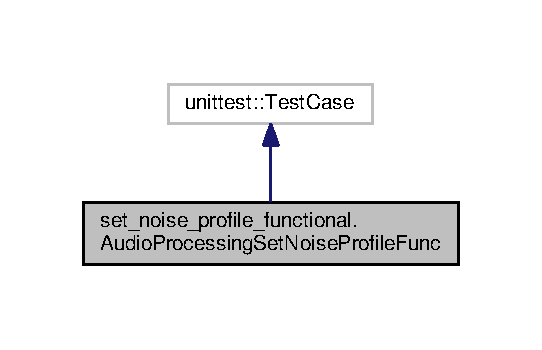
\includegraphics[width=260pt]{classset__noise__profile__functional_1_1AudioProcessingSetNoiseProfileFunc__inherit__graph}
\end{center}
\end{figure}


Collaboration diagram for set\-\_\-noise\-\_\-profile\-\_\-functional.\-Audio\-Processing\-Set\-Noise\-Profile\-Func\-:
\nopagebreak
\begin{figure}[H]
\begin{center}
\leavevmode
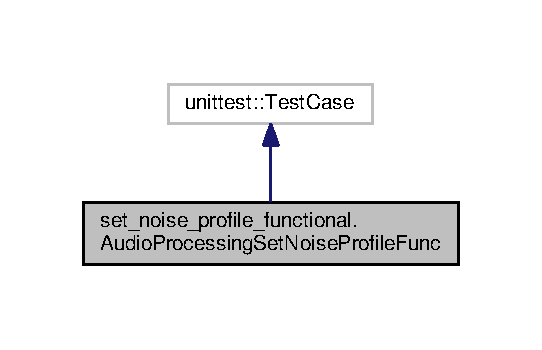
\includegraphics[width=260pt]{classset__noise__profile__functional_1_1AudioProcessingSetNoiseProfileFunc__coll__graph}
\end{center}
\end{figure}
\subsection*{Public Member Functions}
\begin{DoxyCompactItemize}
\item 
def \hyperlink{classset__noise__profile__functional_1_1AudioProcessingSetNoiseProfileFunc_a3ef448c951814ca99645f5ff4a85e851}{test\-\_\-set\-Noise\-Profile\-Service\-\_\-no\-\_\-silence\-\_\-file}
\item 
def \hyperlink{classset__noise__profile__functional_1_1AudioProcessingSetNoiseProfileFunc_ad2eae45e356d7e357a61cf063282b436}{test\-\_\-set\-Noise\-Profile\-Service\-\_\-ogg}
\item 
def \hyperlink{classset__noise__profile__functional_1_1AudioProcessingSetNoiseProfileFunc_a488cabdfe725f1a993a42b7d8c6776d0}{test\-\_\-set\-Noise\-Profile\-Service\-\_\-ogg\-\_\-stress}
\item 
def \hyperlink{classset__noise__profile__functional_1_1AudioProcessingSetNoiseProfileFunc_a0e02d0dbae0d788d73b8170a9d48650b}{test\-\_\-set\-Noise\-Profile\-Service\-\_\-wav\-\_\-1\-\_\-ch}
\item 
def \hyperlink{classset__noise__profile__functional_1_1AudioProcessingSetNoiseProfileFunc_a84cd05103322edf9ed9290785b3493b4}{test\-\_\-set\-Noise\-Profile\-Service\-\_\-wav\-\_\-4\-\_\-ch}
\item 
def \hyperlink{classset__noise__profile__functional_1_1AudioProcessingSetNoiseProfileFunc_a263ecbeb3db73f82958ef45b68a9db30}{test\-\_\-set\-Noise\-Profile\-Service\-\_\-wav\-\_\-6\-\_\-ch}
\end{DoxyCompactItemize}


\subsection{Detailed Description}


Definition at line 35 of file set\-\_\-noise\-\_\-profile\-\_\-functional.\-py.



\subsection{Member Function Documentation}
\hypertarget{classset__noise__profile__functional_1_1AudioProcessingSetNoiseProfileFunc_a3ef448c951814ca99645f5ff4a85e851}{\index{set\-\_\-noise\-\_\-profile\-\_\-functional\-::\-Audio\-Processing\-Set\-Noise\-Profile\-Func@{set\-\_\-noise\-\_\-profile\-\_\-functional\-::\-Audio\-Processing\-Set\-Noise\-Profile\-Func}!test\-\_\-set\-Noise\-Profile\-Service\-\_\-no\-\_\-silence\-\_\-file@{test\-\_\-set\-Noise\-Profile\-Service\-\_\-no\-\_\-silence\-\_\-file}}
\index{test\-\_\-set\-Noise\-Profile\-Service\-\_\-no\-\_\-silence\-\_\-file@{test\-\_\-set\-Noise\-Profile\-Service\-\_\-no\-\_\-silence\-\_\-file}!set_noise_profile_functional::AudioProcessingSetNoiseProfileFunc@{set\-\_\-noise\-\_\-profile\-\_\-functional\-::\-Audio\-Processing\-Set\-Noise\-Profile\-Func}}
\subsubsection[{test\-\_\-set\-Noise\-Profile\-Service\-\_\-no\-\_\-silence\-\_\-file}]{\setlength{\rightskip}{0pt plus 5cm}def set\-\_\-noise\-\_\-profile\-\_\-functional.\-Audio\-Processing\-Set\-Noise\-Profile\-Func.\-test\-\_\-set\-Noise\-Profile\-Service\-\_\-no\-\_\-silence\-\_\-file (
\begin{DoxyParamCaption}
\item[{}]{self}
\end{DoxyParamCaption}
)}}\label{classset__noise__profile__functional_1_1AudioProcessingSetNoiseProfileFunc_a3ef448c951814ca99645f5ff4a85e851}


Definition at line 122 of file set\-\_\-noise\-\_\-profile\-\_\-functional.\-py.

\hypertarget{classset__noise__profile__functional_1_1AudioProcessingSetNoiseProfileFunc_ad2eae45e356d7e357a61cf063282b436}{\index{set\-\_\-noise\-\_\-profile\-\_\-functional\-::\-Audio\-Processing\-Set\-Noise\-Profile\-Func@{set\-\_\-noise\-\_\-profile\-\_\-functional\-::\-Audio\-Processing\-Set\-Noise\-Profile\-Func}!test\-\_\-set\-Noise\-Profile\-Service\-\_\-ogg@{test\-\_\-set\-Noise\-Profile\-Service\-\_\-ogg}}
\index{test\-\_\-set\-Noise\-Profile\-Service\-\_\-ogg@{test\-\_\-set\-Noise\-Profile\-Service\-\_\-ogg}!set_noise_profile_functional::AudioProcessingSetNoiseProfileFunc@{set\-\_\-noise\-\_\-profile\-\_\-functional\-::\-Audio\-Processing\-Set\-Noise\-Profile\-Func}}
\subsubsection[{test\-\_\-set\-Noise\-Profile\-Service\-\_\-ogg}]{\setlength{\rightskip}{0pt plus 5cm}def set\-\_\-noise\-\_\-profile\-\_\-functional.\-Audio\-Processing\-Set\-Noise\-Profile\-Func.\-test\-\_\-set\-Noise\-Profile\-Service\-\_\-ogg (
\begin{DoxyParamCaption}
\item[{}]{self}
\end{DoxyParamCaption}
)}}\label{classset__noise__profile__functional_1_1AudioProcessingSetNoiseProfileFunc_ad2eae45e356d7e357a61cf063282b436}


Definition at line 37 of file set\-\_\-noise\-\_\-profile\-\_\-functional.\-py.

\hypertarget{classset__noise__profile__functional_1_1AudioProcessingSetNoiseProfileFunc_a488cabdfe725f1a993a42b7d8c6776d0}{\index{set\-\_\-noise\-\_\-profile\-\_\-functional\-::\-Audio\-Processing\-Set\-Noise\-Profile\-Func@{set\-\_\-noise\-\_\-profile\-\_\-functional\-::\-Audio\-Processing\-Set\-Noise\-Profile\-Func}!test\-\_\-set\-Noise\-Profile\-Service\-\_\-ogg\-\_\-stress@{test\-\_\-set\-Noise\-Profile\-Service\-\_\-ogg\-\_\-stress}}
\index{test\-\_\-set\-Noise\-Profile\-Service\-\_\-ogg\-\_\-stress@{test\-\_\-set\-Noise\-Profile\-Service\-\_\-ogg\-\_\-stress}!set_noise_profile_functional::AudioProcessingSetNoiseProfileFunc@{set\-\_\-noise\-\_\-profile\-\_\-functional\-::\-Audio\-Processing\-Set\-Noise\-Profile\-Func}}
\subsubsection[{test\-\_\-set\-Noise\-Profile\-Service\-\_\-ogg\-\_\-stress}]{\setlength{\rightskip}{0pt plus 5cm}def set\-\_\-noise\-\_\-profile\-\_\-functional.\-Audio\-Processing\-Set\-Noise\-Profile\-Func.\-test\-\_\-set\-Noise\-Profile\-Service\-\_\-ogg\-\_\-stress (
\begin{DoxyParamCaption}
\item[{}]{self}
\end{DoxyParamCaption}
)}}\label{classset__noise__profile__functional_1_1AudioProcessingSetNoiseProfileFunc_a488cabdfe725f1a993a42b7d8c6776d0}


Definition at line 55 of file set\-\_\-noise\-\_\-profile\-\_\-functional.\-py.

\hypertarget{classset__noise__profile__functional_1_1AudioProcessingSetNoiseProfileFunc_a0e02d0dbae0d788d73b8170a9d48650b}{\index{set\-\_\-noise\-\_\-profile\-\_\-functional\-::\-Audio\-Processing\-Set\-Noise\-Profile\-Func@{set\-\_\-noise\-\_\-profile\-\_\-functional\-::\-Audio\-Processing\-Set\-Noise\-Profile\-Func}!test\-\_\-set\-Noise\-Profile\-Service\-\_\-wav\-\_\-1\-\_\-ch@{test\-\_\-set\-Noise\-Profile\-Service\-\_\-wav\-\_\-1\-\_\-ch}}
\index{test\-\_\-set\-Noise\-Profile\-Service\-\_\-wav\-\_\-1\-\_\-ch@{test\-\_\-set\-Noise\-Profile\-Service\-\_\-wav\-\_\-1\-\_\-ch}!set_noise_profile_functional::AudioProcessingSetNoiseProfileFunc@{set\-\_\-noise\-\_\-profile\-\_\-functional\-::\-Audio\-Processing\-Set\-Noise\-Profile\-Func}}
\subsubsection[{test\-\_\-set\-Noise\-Profile\-Service\-\_\-wav\-\_\-1\-\_\-ch}]{\setlength{\rightskip}{0pt plus 5cm}def set\-\_\-noise\-\_\-profile\-\_\-functional.\-Audio\-Processing\-Set\-Noise\-Profile\-Func.\-test\-\_\-set\-Noise\-Profile\-Service\-\_\-wav\-\_\-1\-\_\-ch (
\begin{DoxyParamCaption}
\item[{}]{self}
\end{DoxyParamCaption}
)}}\label{classset__noise__profile__functional_1_1AudioProcessingSetNoiseProfileFunc_a0e02d0dbae0d788d73b8170a9d48650b}


Definition at line 74 of file set\-\_\-noise\-\_\-profile\-\_\-functional.\-py.

\hypertarget{classset__noise__profile__functional_1_1AudioProcessingSetNoiseProfileFunc_a84cd05103322edf9ed9290785b3493b4}{\index{set\-\_\-noise\-\_\-profile\-\_\-functional\-::\-Audio\-Processing\-Set\-Noise\-Profile\-Func@{set\-\_\-noise\-\_\-profile\-\_\-functional\-::\-Audio\-Processing\-Set\-Noise\-Profile\-Func}!test\-\_\-set\-Noise\-Profile\-Service\-\_\-wav\-\_\-4\-\_\-ch@{test\-\_\-set\-Noise\-Profile\-Service\-\_\-wav\-\_\-4\-\_\-ch}}
\index{test\-\_\-set\-Noise\-Profile\-Service\-\_\-wav\-\_\-4\-\_\-ch@{test\-\_\-set\-Noise\-Profile\-Service\-\_\-wav\-\_\-4\-\_\-ch}!set_noise_profile_functional::AudioProcessingSetNoiseProfileFunc@{set\-\_\-noise\-\_\-profile\-\_\-functional\-::\-Audio\-Processing\-Set\-Noise\-Profile\-Func}}
\subsubsection[{test\-\_\-set\-Noise\-Profile\-Service\-\_\-wav\-\_\-4\-\_\-ch}]{\setlength{\rightskip}{0pt plus 5cm}def set\-\_\-noise\-\_\-profile\-\_\-functional.\-Audio\-Processing\-Set\-Noise\-Profile\-Func.\-test\-\_\-set\-Noise\-Profile\-Service\-\_\-wav\-\_\-4\-\_\-ch (
\begin{DoxyParamCaption}
\item[{}]{self}
\end{DoxyParamCaption}
)}}\label{classset__noise__profile__functional_1_1AudioProcessingSetNoiseProfileFunc_a84cd05103322edf9ed9290785b3493b4}


Definition at line 90 of file set\-\_\-noise\-\_\-profile\-\_\-functional.\-py.

\hypertarget{classset__noise__profile__functional_1_1AudioProcessingSetNoiseProfileFunc_a263ecbeb3db73f82958ef45b68a9db30}{\index{set\-\_\-noise\-\_\-profile\-\_\-functional\-::\-Audio\-Processing\-Set\-Noise\-Profile\-Func@{set\-\_\-noise\-\_\-profile\-\_\-functional\-::\-Audio\-Processing\-Set\-Noise\-Profile\-Func}!test\-\_\-set\-Noise\-Profile\-Service\-\_\-wav\-\_\-6\-\_\-ch@{test\-\_\-set\-Noise\-Profile\-Service\-\_\-wav\-\_\-6\-\_\-ch}}
\index{test\-\_\-set\-Noise\-Profile\-Service\-\_\-wav\-\_\-6\-\_\-ch@{test\-\_\-set\-Noise\-Profile\-Service\-\_\-wav\-\_\-6\-\_\-ch}!set_noise_profile_functional::AudioProcessingSetNoiseProfileFunc@{set\-\_\-noise\-\_\-profile\-\_\-functional\-::\-Audio\-Processing\-Set\-Noise\-Profile\-Func}}
\subsubsection[{test\-\_\-set\-Noise\-Profile\-Service\-\_\-wav\-\_\-6\-\_\-ch}]{\setlength{\rightskip}{0pt plus 5cm}def set\-\_\-noise\-\_\-profile\-\_\-functional.\-Audio\-Processing\-Set\-Noise\-Profile\-Func.\-test\-\_\-set\-Noise\-Profile\-Service\-\_\-wav\-\_\-6\-\_\-ch (
\begin{DoxyParamCaption}
\item[{}]{self}
\end{DoxyParamCaption}
)}}\label{classset__noise__profile__functional_1_1AudioProcessingSetNoiseProfileFunc_a263ecbeb3db73f82958ef45b68a9db30}


Definition at line 106 of file set\-\_\-noise\-\_\-profile\-\_\-functional.\-py.



The documentation for this class was generated from the following file\-:\begin{DoxyCompactItemize}
\item 
/home/travis/rapp\-\_\-temp/rapp-\/platform/rapp\-\_\-audio\-\_\-processing/tests/functional/\hyperlink{set__noise__profile__functional_8py}{set\-\_\-noise\-\_\-profile\-\_\-functional.\-py}\end{DoxyCompactItemize}

\hypertarget{classdenoise__unit__tests_1_1TestAudioProcessing}{\section{denoise\-\_\-unit\-\_\-tests.\-Test\-Audio\-Processing Class Reference}
\label{classdenoise__unit__tests_1_1TestAudioProcessing}\index{denoise\-\_\-unit\-\_\-tests.\-Test\-Audio\-Processing@{denoise\-\_\-unit\-\_\-tests.\-Test\-Audio\-Processing}}
}


Inheritance diagram for denoise\-\_\-unit\-\_\-tests.\-Test\-Audio\-Processing\-:


Collaboration diagram for denoise\-\_\-unit\-\_\-tests.\-Test\-Audio\-Processing\-:
\subsection*{Public Member Functions}
\begin{DoxyCompactItemize}
\item 
def \hyperlink{classdenoise__unit__tests_1_1TestAudioProcessing_a7de102218fb2997e1ee3eb54f019716b}{set\-Up}
\item 
def \hyperlink{classdenoise__unit__tests_1_1TestAudioProcessing_a0b5ba548d4ed4c51c433e2ec4e3ebe74}{tear\-Down}
\item 
def \hyperlink{classdenoise__unit__tests_1_1TestAudioProcessing_ae1a17e135285902d2d1994b0a3f097b5}{test\-\_\-negative\-Scale}
\item 
def \hyperlink{classdenoise__unit__tests_1_1TestAudioProcessing_abb6cbcda08af0c243a5d561433b32a70}{test\-\_\-not\-Existent\-Audio\-File}
\item 
def \hyperlink{classdenoise__unit__tests_1_1TestAudioProcessing_abef05168d2756e37aed2689423b62402}{test\-\_\-not\-Existent\-Audio\-Type}
\item 
def \hyperlink{classdenoise__unit__tests_1_1TestAudioProcessing_abb7c4de41acad528eb555ffa3f4569a7}{test\-\_\-not\-Existent\-User}
\item 
def \hyperlink{classdenoise__unit__tests_1_1TestAudioProcessing_aa5aa322c8e8c137b2df7abb7b28b8430}{test\-\_\-ogg\-\_\-type\-\_\-wav\-\_\-1\-\_\-ch\-\_\-file}
\item 
def \hyperlink{classdenoise__unit__tests_1_1TestAudioProcessing_a8ab2e76b611895890ba4e5e0894a4437}{test\-\_\-ogg\-\_\-type\-\_\-wav\-\_\-4\-\_\-ch\-\_\-file}
\item 
def \hyperlink{classdenoise__unit__tests_1_1TestAudioProcessing_aec16b59a6ea0211f8fd79d4ca4d68cb4}{test\-\_\-real\-File}
\item 
def \hyperlink{classdenoise__unit__tests_1_1TestAudioProcessing_a0a82f099904bbeec84a9416b5c8b9af6}{test\-\_\-wav\-\_\-1\-\_\-ch\-\_\-type\-\_\-ogg\-\_\-file}
\item 
def \hyperlink{classdenoise__unit__tests_1_1TestAudioProcessing_a9ac397525cbf072a7b5c7507cfc3f850}{test\-\_\-wav\-\_\-1\-\_\-ch\-\_\-type\-\_\-wav\-\_\-4\-\_\-ch\-\_\-file}
\item 
def \hyperlink{classdenoise__unit__tests_1_1TestAudioProcessing_aedebea8664cc5588c78083fd4cb00ffa}{test\-\_\-wav\-\_\-4\-\_\-ch\-\_\-type\-\_\-ogg\-\_\-file}
\item 
def \hyperlink{classdenoise__unit__tests_1_1TestAudioProcessing_a1592faaf83d011ff61520ad7dbac9875}{test\-\_\-wav\-\_\-4\-\_\-ch\-\_\-type\-\_\-wav\-\_\-1\-\_\-ch\-\_\-file}
\end{DoxyCompactItemize}
\subsection*{Public Attributes}
\begin{DoxyCompactItemize}
\item 
\hyperlink{classdenoise__unit__tests_1_1TestAudioProcessing_a40e5a23bc69a679a00dee88b7992a790}{auxiliary\-\_\-files\-\_\-url}
\item 
\hyperlink{classdenoise__unit__tests_1_1TestAudioProcessing_abd4c388e17fb4ffedf516e1e0b8684a4}{rospack}
\item 
\hyperlink{classdenoise__unit__tests_1_1TestAudioProcessing_a03ae317aea198943ba8f162aee887cc3}{sox\-\_\-denoise\-\_\-module}
\end{DoxyCompactItemize}


\subsection{Detailed Description}


Definition at line 33 of file denoise\-\_\-unit\-\_\-tests.\-py.



\subsection{Member Function Documentation}
\hypertarget{classdenoise__unit__tests_1_1TestAudioProcessing_a7de102218fb2997e1ee3eb54f019716b}{\index{denoise\-\_\-unit\-\_\-tests\-::\-Test\-Audio\-Processing@{denoise\-\_\-unit\-\_\-tests\-::\-Test\-Audio\-Processing}!set\-Up@{set\-Up}}
\index{set\-Up@{set\-Up}!denoise_unit_tests::TestAudioProcessing@{denoise\-\_\-unit\-\_\-tests\-::\-Test\-Audio\-Processing}}
\subsubsection[{set\-Up}]{\setlength{\rightskip}{0pt plus 5cm}def denoise\-\_\-unit\-\_\-tests.\-Test\-Audio\-Processing.\-set\-Up (
\begin{DoxyParamCaption}
\item[{}]{self}
\end{DoxyParamCaption}
)}}\label{classdenoise__unit__tests_1_1TestAudioProcessing_a7de102218fb2997e1ee3eb54f019716b}


Definition at line 34 of file denoise\-\_\-unit\-\_\-tests.\-py.

\hypertarget{classdenoise__unit__tests_1_1TestAudioProcessing_a0b5ba548d4ed4c51c433e2ec4e3ebe74}{\index{denoise\-\_\-unit\-\_\-tests\-::\-Test\-Audio\-Processing@{denoise\-\_\-unit\-\_\-tests\-::\-Test\-Audio\-Processing}!tear\-Down@{tear\-Down}}
\index{tear\-Down@{tear\-Down}!denoise_unit_tests::TestAudioProcessing@{denoise\-\_\-unit\-\_\-tests\-::\-Test\-Audio\-Processing}}
\subsubsection[{tear\-Down}]{\setlength{\rightskip}{0pt plus 5cm}def denoise\-\_\-unit\-\_\-tests.\-Test\-Audio\-Processing.\-tear\-Down (
\begin{DoxyParamCaption}
\item[{}]{self}
\end{DoxyParamCaption}
)}}\label{classdenoise__unit__tests_1_1TestAudioProcessing_a0b5ba548d4ed4c51c433e2ec4e3ebe74}


Definition at line 40 of file denoise\-\_\-unit\-\_\-tests.\-py.

\hypertarget{classdenoise__unit__tests_1_1TestAudioProcessing_ae1a17e135285902d2d1994b0a3f097b5}{\index{denoise\-\_\-unit\-\_\-tests\-::\-Test\-Audio\-Processing@{denoise\-\_\-unit\-\_\-tests\-::\-Test\-Audio\-Processing}!test\-\_\-negative\-Scale@{test\-\_\-negative\-Scale}}
\index{test\-\_\-negative\-Scale@{test\-\_\-negative\-Scale}!denoise_unit_tests::TestAudioProcessing@{denoise\-\_\-unit\-\_\-tests\-::\-Test\-Audio\-Processing}}
\subsubsection[{test\-\_\-negative\-Scale}]{\setlength{\rightskip}{0pt plus 5cm}def denoise\-\_\-unit\-\_\-tests.\-Test\-Audio\-Processing.\-test\-\_\-negative\-Scale (
\begin{DoxyParamCaption}
\item[{}]{self}
\end{DoxyParamCaption}
)}}\label{classdenoise__unit__tests_1_1TestAudioProcessing_ae1a17e135285902d2d1994b0a3f097b5}


Definition at line 123 of file denoise\-\_\-unit\-\_\-tests.\-py.

\hypertarget{classdenoise__unit__tests_1_1TestAudioProcessing_abb6cbcda08af0c243a5d561433b32a70}{\index{denoise\-\_\-unit\-\_\-tests\-::\-Test\-Audio\-Processing@{denoise\-\_\-unit\-\_\-tests\-::\-Test\-Audio\-Processing}!test\-\_\-not\-Existent\-Audio\-File@{test\-\_\-not\-Existent\-Audio\-File}}
\index{test\-\_\-not\-Existent\-Audio\-File@{test\-\_\-not\-Existent\-Audio\-File}!denoise_unit_tests::TestAudioProcessing@{denoise\-\_\-unit\-\_\-tests\-::\-Test\-Audio\-Processing}}
\subsubsection[{test\-\_\-not\-Existent\-Audio\-File}]{\setlength{\rightskip}{0pt plus 5cm}def denoise\-\_\-unit\-\_\-tests.\-Test\-Audio\-Processing.\-test\-\_\-not\-Existent\-Audio\-File (
\begin{DoxyParamCaption}
\item[{}]{self}
\end{DoxyParamCaption}
)}}\label{classdenoise__unit__tests_1_1TestAudioProcessing_abb6cbcda08af0c243a5d561433b32a70}


Definition at line 76 of file denoise\-\_\-unit\-\_\-tests.\-py.

\hypertarget{classdenoise__unit__tests_1_1TestAudioProcessing_abef05168d2756e37aed2689423b62402}{\index{denoise\-\_\-unit\-\_\-tests\-::\-Test\-Audio\-Processing@{denoise\-\_\-unit\-\_\-tests\-::\-Test\-Audio\-Processing}!test\-\_\-not\-Existent\-Audio\-Type@{test\-\_\-not\-Existent\-Audio\-Type}}
\index{test\-\_\-not\-Existent\-Audio\-Type@{test\-\_\-not\-Existent\-Audio\-Type}!denoise_unit_tests::TestAudioProcessing@{denoise\-\_\-unit\-\_\-tests\-::\-Test\-Audio\-Processing}}
\subsubsection[{test\-\_\-not\-Existent\-Audio\-Type}]{\setlength{\rightskip}{0pt plus 5cm}def denoise\-\_\-unit\-\_\-tests.\-Test\-Audio\-Processing.\-test\-\_\-not\-Existent\-Audio\-Type (
\begin{DoxyParamCaption}
\item[{}]{self}
\end{DoxyParamCaption}
)}}\label{classdenoise__unit__tests_1_1TestAudioProcessing_abef05168d2756e37aed2689423b62402}


Definition at line 108 of file denoise\-\_\-unit\-\_\-tests.\-py.

\hypertarget{classdenoise__unit__tests_1_1TestAudioProcessing_abb7c4de41acad528eb555ffa3f4569a7}{\index{denoise\-\_\-unit\-\_\-tests\-::\-Test\-Audio\-Processing@{denoise\-\_\-unit\-\_\-tests\-::\-Test\-Audio\-Processing}!test\-\_\-not\-Existent\-User@{test\-\_\-not\-Existent\-User}}
\index{test\-\_\-not\-Existent\-User@{test\-\_\-not\-Existent\-User}!denoise_unit_tests::TestAudioProcessing@{denoise\-\_\-unit\-\_\-tests\-::\-Test\-Audio\-Processing}}
\subsubsection[{test\-\_\-not\-Existent\-User}]{\setlength{\rightskip}{0pt plus 5cm}def denoise\-\_\-unit\-\_\-tests.\-Test\-Audio\-Processing.\-test\-\_\-not\-Existent\-User (
\begin{DoxyParamCaption}
\item[{}]{self}
\end{DoxyParamCaption}
)}}\label{classdenoise__unit__tests_1_1TestAudioProcessing_abb7c4de41acad528eb555ffa3f4569a7}


Definition at line 92 of file denoise\-\_\-unit\-\_\-tests.\-py.

\hypertarget{classdenoise__unit__tests_1_1TestAudioProcessing_aa5aa322c8e8c137b2df7abb7b28b8430}{\index{denoise\-\_\-unit\-\_\-tests\-::\-Test\-Audio\-Processing@{denoise\-\_\-unit\-\_\-tests\-::\-Test\-Audio\-Processing}!test\-\_\-ogg\-\_\-type\-\_\-wav\-\_\-1\-\_\-ch\-\_\-file@{test\-\_\-ogg\-\_\-type\-\_\-wav\-\_\-1\-\_\-ch\-\_\-file}}
\index{test\-\_\-ogg\-\_\-type\-\_\-wav\-\_\-1\-\_\-ch\-\_\-file@{test\-\_\-ogg\-\_\-type\-\_\-wav\-\_\-1\-\_\-ch\-\_\-file}!denoise_unit_tests::TestAudioProcessing@{denoise\-\_\-unit\-\_\-tests\-::\-Test\-Audio\-Processing}}
\subsubsection[{test\-\_\-ogg\-\_\-type\-\_\-wav\-\_\-1\-\_\-ch\-\_\-file}]{\setlength{\rightskip}{0pt plus 5cm}def denoise\-\_\-unit\-\_\-tests.\-Test\-Audio\-Processing.\-test\-\_\-ogg\-\_\-type\-\_\-wav\-\_\-1\-\_\-ch\-\_\-file (
\begin{DoxyParamCaption}
\item[{}]{self}
\end{DoxyParamCaption}
)}}\label{classdenoise__unit__tests_1_1TestAudioProcessing_aa5aa322c8e8c137b2df7abb7b28b8430}


Definition at line 138 of file denoise\-\_\-unit\-\_\-tests.\-py.

\hypertarget{classdenoise__unit__tests_1_1TestAudioProcessing_a8ab2e76b611895890ba4e5e0894a4437}{\index{denoise\-\_\-unit\-\_\-tests\-::\-Test\-Audio\-Processing@{denoise\-\_\-unit\-\_\-tests\-::\-Test\-Audio\-Processing}!test\-\_\-ogg\-\_\-type\-\_\-wav\-\_\-4\-\_\-ch\-\_\-file@{test\-\_\-ogg\-\_\-type\-\_\-wav\-\_\-4\-\_\-ch\-\_\-file}}
\index{test\-\_\-ogg\-\_\-type\-\_\-wav\-\_\-4\-\_\-ch\-\_\-file@{test\-\_\-ogg\-\_\-type\-\_\-wav\-\_\-4\-\_\-ch\-\_\-file}!denoise_unit_tests::TestAudioProcessing@{denoise\-\_\-unit\-\_\-tests\-::\-Test\-Audio\-Processing}}
\subsubsection[{test\-\_\-ogg\-\_\-type\-\_\-wav\-\_\-4\-\_\-ch\-\_\-file}]{\setlength{\rightskip}{0pt plus 5cm}def denoise\-\_\-unit\-\_\-tests.\-Test\-Audio\-Processing.\-test\-\_\-ogg\-\_\-type\-\_\-wav\-\_\-4\-\_\-ch\-\_\-file (
\begin{DoxyParamCaption}
\item[{}]{self}
\end{DoxyParamCaption}
)}}\label{classdenoise__unit__tests_1_1TestAudioProcessing_a8ab2e76b611895890ba4e5e0894a4437}


Definition at line 153 of file denoise\-\_\-unit\-\_\-tests.\-py.

\hypertarget{classdenoise__unit__tests_1_1TestAudioProcessing_aec16b59a6ea0211f8fd79d4ca4d68cb4}{\index{denoise\-\_\-unit\-\_\-tests\-::\-Test\-Audio\-Processing@{denoise\-\_\-unit\-\_\-tests\-::\-Test\-Audio\-Processing}!test\-\_\-real\-File@{test\-\_\-real\-File}}
\index{test\-\_\-real\-File@{test\-\_\-real\-File}!denoise_unit_tests::TestAudioProcessing@{denoise\-\_\-unit\-\_\-tests\-::\-Test\-Audio\-Processing}}
\subsubsection[{test\-\_\-real\-File}]{\setlength{\rightskip}{0pt plus 5cm}def denoise\-\_\-unit\-\_\-tests.\-Test\-Audio\-Processing.\-test\-\_\-real\-File (
\begin{DoxyParamCaption}
\item[{}]{self}
\end{DoxyParamCaption}
)}}\label{classdenoise__unit__tests_1_1TestAudioProcessing_aec16b59a6ea0211f8fd79d4ca4d68cb4}


Definition at line 44 of file denoise\-\_\-unit\-\_\-tests.\-py.

\hypertarget{classdenoise__unit__tests_1_1TestAudioProcessing_a0a82f099904bbeec84a9416b5c8b9af6}{\index{denoise\-\_\-unit\-\_\-tests\-::\-Test\-Audio\-Processing@{denoise\-\_\-unit\-\_\-tests\-::\-Test\-Audio\-Processing}!test\-\_\-wav\-\_\-1\-\_\-ch\-\_\-type\-\_\-ogg\-\_\-file@{test\-\_\-wav\-\_\-1\-\_\-ch\-\_\-type\-\_\-ogg\-\_\-file}}
\index{test\-\_\-wav\-\_\-1\-\_\-ch\-\_\-type\-\_\-ogg\-\_\-file@{test\-\_\-wav\-\_\-1\-\_\-ch\-\_\-type\-\_\-ogg\-\_\-file}!denoise_unit_tests::TestAudioProcessing@{denoise\-\_\-unit\-\_\-tests\-::\-Test\-Audio\-Processing}}
\subsubsection[{test\-\_\-wav\-\_\-1\-\_\-ch\-\_\-type\-\_\-ogg\-\_\-file}]{\setlength{\rightskip}{0pt plus 5cm}def denoise\-\_\-unit\-\_\-tests.\-Test\-Audio\-Processing.\-test\-\_\-wav\-\_\-1\-\_\-ch\-\_\-type\-\_\-ogg\-\_\-file (
\begin{DoxyParamCaption}
\item[{}]{self}
\end{DoxyParamCaption}
)}}\label{classdenoise__unit__tests_1_1TestAudioProcessing_a0a82f099904bbeec84a9416b5c8b9af6}


Definition at line 168 of file denoise\-\_\-unit\-\_\-tests.\-py.

\hypertarget{classdenoise__unit__tests_1_1TestAudioProcessing_a9ac397525cbf072a7b5c7507cfc3f850}{\index{denoise\-\_\-unit\-\_\-tests\-::\-Test\-Audio\-Processing@{denoise\-\_\-unit\-\_\-tests\-::\-Test\-Audio\-Processing}!test\-\_\-wav\-\_\-1\-\_\-ch\-\_\-type\-\_\-wav\-\_\-4\-\_\-ch\-\_\-file@{test\-\_\-wav\-\_\-1\-\_\-ch\-\_\-type\-\_\-wav\-\_\-4\-\_\-ch\-\_\-file}}
\index{test\-\_\-wav\-\_\-1\-\_\-ch\-\_\-type\-\_\-wav\-\_\-4\-\_\-ch\-\_\-file@{test\-\_\-wav\-\_\-1\-\_\-ch\-\_\-type\-\_\-wav\-\_\-4\-\_\-ch\-\_\-file}!denoise_unit_tests::TestAudioProcessing@{denoise\-\_\-unit\-\_\-tests\-::\-Test\-Audio\-Processing}}
\subsubsection[{test\-\_\-wav\-\_\-1\-\_\-ch\-\_\-type\-\_\-wav\-\_\-4\-\_\-ch\-\_\-file}]{\setlength{\rightskip}{0pt plus 5cm}def denoise\-\_\-unit\-\_\-tests.\-Test\-Audio\-Processing.\-test\-\_\-wav\-\_\-1\-\_\-ch\-\_\-type\-\_\-wav\-\_\-4\-\_\-ch\-\_\-file (
\begin{DoxyParamCaption}
\item[{}]{self}
\end{DoxyParamCaption}
)}}\label{classdenoise__unit__tests_1_1TestAudioProcessing_a9ac397525cbf072a7b5c7507cfc3f850}


Definition at line 183 of file denoise\-\_\-unit\-\_\-tests.\-py.

\hypertarget{classdenoise__unit__tests_1_1TestAudioProcessing_aedebea8664cc5588c78083fd4cb00ffa}{\index{denoise\-\_\-unit\-\_\-tests\-::\-Test\-Audio\-Processing@{denoise\-\_\-unit\-\_\-tests\-::\-Test\-Audio\-Processing}!test\-\_\-wav\-\_\-4\-\_\-ch\-\_\-type\-\_\-ogg\-\_\-file@{test\-\_\-wav\-\_\-4\-\_\-ch\-\_\-type\-\_\-ogg\-\_\-file}}
\index{test\-\_\-wav\-\_\-4\-\_\-ch\-\_\-type\-\_\-ogg\-\_\-file@{test\-\_\-wav\-\_\-4\-\_\-ch\-\_\-type\-\_\-ogg\-\_\-file}!denoise_unit_tests::TestAudioProcessing@{denoise\-\_\-unit\-\_\-tests\-::\-Test\-Audio\-Processing}}
\subsubsection[{test\-\_\-wav\-\_\-4\-\_\-ch\-\_\-type\-\_\-ogg\-\_\-file}]{\setlength{\rightskip}{0pt plus 5cm}def denoise\-\_\-unit\-\_\-tests.\-Test\-Audio\-Processing.\-test\-\_\-wav\-\_\-4\-\_\-ch\-\_\-type\-\_\-ogg\-\_\-file (
\begin{DoxyParamCaption}
\item[{}]{self}
\end{DoxyParamCaption}
)}}\label{classdenoise__unit__tests_1_1TestAudioProcessing_aedebea8664cc5588c78083fd4cb00ffa}


Definition at line 198 of file denoise\-\_\-unit\-\_\-tests.\-py.

\hypertarget{classdenoise__unit__tests_1_1TestAudioProcessing_a1592faaf83d011ff61520ad7dbac9875}{\index{denoise\-\_\-unit\-\_\-tests\-::\-Test\-Audio\-Processing@{denoise\-\_\-unit\-\_\-tests\-::\-Test\-Audio\-Processing}!test\-\_\-wav\-\_\-4\-\_\-ch\-\_\-type\-\_\-wav\-\_\-1\-\_\-ch\-\_\-file@{test\-\_\-wav\-\_\-4\-\_\-ch\-\_\-type\-\_\-wav\-\_\-1\-\_\-ch\-\_\-file}}
\index{test\-\_\-wav\-\_\-4\-\_\-ch\-\_\-type\-\_\-wav\-\_\-1\-\_\-ch\-\_\-file@{test\-\_\-wav\-\_\-4\-\_\-ch\-\_\-type\-\_\-wav\-\_\-1\-\_\-ch\-\_\-file}!denoise_unit_tests::TestAudioProcessing@{denoise\-\_\-unit\-\_\-tests\-::\-Test\-Audio\-Processing}}
\subsubsection[{test\-\_\-wav\-\_\-4\-\_\-ch\-\_\-type\-\_\-wav\-\_\-1\-\_\-ch\-\_\-file}]{\setlength{\rightskip}{0pt plus 5cm}def denoise\-\_\-unit\-\_\-tests.\-Test\-Audio\-Processing.\-test\-\_\-wav\-\_\-4\-\_\-ch\-\_\-type\-\_\-wav\-\_\-1\-\_\-ch\-\_\-file (
\begin{DoxyParamCaption}
\item[{}]{self}
\end{DoxyParamCaption}
)}}\label{classdenoise__unit__tests_1_1TestAudioProcessing_a1592faaf83d011ff61520ad7dbac9875}


Definition at line 213 of file denoise\-\_\-unit\-\_\-tests.\-py.



\subsection{Member Data Documentation}
\hypertarget{classdenoise__unit__tests_1_1TestAudioProcessing_a40e5a23bc69a679a00dee88b7992a790}{\index{denoise\-\_\-unit\-\_\-tests\-::\-Test\-Audio\-Processing@{denoise\-\_\-unit\-\_\-tests\-::\-Test\-Audio\-Processing}!auxiliary\-\_\-files\-\_\-url@{auxiliary\-\_\-files\-\_\-url}}
\index{auxiliary\-\_\-files\-\_\-url@{auxiliary\-\_\-files\-\_\-url}!denoise_unit_tests::TestAudioProcessing@{denoise\-\_\-unit\-\_\-tests\-::\-Test\-Audio\-Processing}}
\subsubsection[{auxiliary\-\_\-files\-\_\-url}]{\setlength{\rightskip}{0pt plus 5cm}denoise\-\_\-unit\-\_\-tests.\-Test\-Audio\-Processing.\-auxiliary\-\_\-files\-\_\-url}}\label{classdenoise__unit__tests_1_1TestAudioProcessing_a40e5a23bc69a679a00dee88b7992a790}


Definition at line 36 of file denoise\-\_\-unit\-\_\-tests.\-py.

\hypertarget{classdenoise__unit__tests_1_1TestAudioProcessing_abd4c388e17fb4ffedf516e1e0b8684a4}{\index{denoise\-\_\-unit\-\_\-tests\-::\-Test\-Audio\-Processing@{denoise\-\_\-unit\-\_\-tests\-::\-Test\-Audio\-Processing}!rospack@{rospack}}
\index{rospack@{rospack}!denoise_unit_tests::TestAudioProcessing@{denoise\-\_\-unit\-\_\-tests\-::\-Test\-Audio\-Processing}}
\subsubsection[{rospack}]{\setlength{\rightskip}{0pt plus 5cm}denoise\-\_\-unit\-\_\-tests.\-Test\-Audio\-Processing.\-rospack}}\label{classdenoise__unit__tests_1_1TestAudioProcessing_abd4c388e17fb4ffedf516e1e0b8684a4}


Definition at line 42 of file denoise\-\_\-unit\-\_\-tests.\-py.

\hypertarget{classdenoise__unit__tests_1_1TestAudioProcessing_a03ae317aea198943ba8f162aee887cc3}{\index{denoise\-\_\-unit\-\_\-tests\-::\-Test\-Audio\-Processing@{denoise\-\_\-unit\-\_\-tests\-::\-Test\-Audio\-Processing}!sox\-\_\-denoise\-\_\-module@{sox\-\_\-denoise\-\_\-module}}
\index{sox\-\_\-denoise\-\_\-module@{sox\-\_\-denoise\-\_\-module}!denoise_unit_tests::TestAudioProcessing@{denoise\-\_\-unit\-\_\-tests\-::\-Test\-Audio\-Processing}}
\subsubsection[{sox\-\_\-denoise\-\_\-module}]{\setlength{\rightskip}{0pt plus 5cm}denoise\-\_\-unit\-\_\-tests.\-Test\-Audio\-Processing.\-sox\-\_\-denoise\-\_\-module}}\label{classdenoise__unit__tests_1_1TestAudioProcessing_a03ae317aea198943ba8f162aee887cc3}


Definition at line 38 of file denoise\-\_\-unit\-\_\-tests.\-py.



The documentation for this class was generated from the following file\-:\begin{DoxyCompactItemize}
\item 
/home/travis/rapp\-\_\-temp/rapp-\/platform/rapp\-\_\-audio\-\_\-processing/tests/unit/\hyperlink{denoise__unit__tests_8py}{denoise\-\_\-unit\-\_\-tests.\-py}\end{DoxyCompactItemize}

\hypertarget{classutilities__unit__tests_1_1TestAudioProcessing}{\section{utilities\-\_\-unit\-\_\-tests.\-Test\-Audio\-Processing Class Reference}
\label{classutilities__unit__tests_1_1TestAudioProcessing}\index{utilities\-\_\-unit\-\_\-tests.\-Test\-Audio\-Processing@{utilities\-\_\-unit\-\_\-tests.\-Test\-Audio\-Processing}}
}


Inheritance diagram for utilities\-\_\-unit\-\_\-tests.\-Test\-Audio\-Processing\-:


Collaboration diagram for utilities\-\_\-unit\-\_\-tests.\-Test\-Audio\-Processing\-:
\subsection*{Public Member Functions}
\begin{DoxyCompactItemize}
\item 
def \hyperlink{classutilities__unit__tests_1_1TestAudioProcessing_a64e2426fc2a035849341bf3583280b44}{set\-Up}
\item 
def \hyperlink{classutilities__unit__tests_1_1TestAudioProcessing_aec5f7490f917d74954baabeb4981027b}{tear\-Down}
\item 
def \hyperlink{classutilities__unit__tests_1_1TestAudioProcessing_aeda2f9f156cf866e541b4f9f4ffd7dc7}{test\-\_\-existent\-Files}
\item 
def \hyperlink{classutilities__unit__tests_1_1TestAudioProcessing_a2450e3d718cbb9f5c365f7dc11875df3}{test\-\_\-mixed\-Cases}
\item 
def \hyperlink{classutilities__unit__tests_1_1TestAudioProcessing_a39c6e0913b06620a9e7118b5021c1cb7}{test\-\_\-not\-Existent\-Files}
\end{DoxyCompactItemize}
\subsection*{Public Attributes}
\begin{DoxyCompactItemize}
\item 
\hyperlink{classutilities__unit__tests_1_1TestAudioProcessing_a8f0150434b471b9822c2d6ff1f89ca4f}{utilities\-\_\-module}
\end{DoxyCompactItemize}


\subsection{Detailed Description}


Definition at line 30 of file utilities\-\_\-unit\-\_\-tests.\-py.



\subsection{Member Function Documentation}
\hypertarget{classutilities__unit__tests_1_1TestAudioProcessing_a64e2426fc2a035849341bf3583280b44}{\index{utilities\-\_\-unit\-\_\-tests\-::\-Test\-Audio\-Processing@{utilities\-\_\-unit\-\_\-tests\-::\-Test\-Audio\-Processing}!set\-Up@{set\-Up}}
\index{set\-Up@{set\-Up}!utilities_unit_tests::TestAudioProcessing@{utilities\-\_\-unit\-\_\-tests\-::\-Test\-Audio\-Processing}}
\subsubsection[{set\-Up}]{\setlength{\rightskip}{0pt plus 5cm}def utilities\-\_\-unit\-\_\-tests.\-Test\-Audio\-Processing.\-set\-Up (
\begin{DoxyParamCaption}
\item[{}]{self}
\end{DoxyParamCaption}
)}}\label{classutilities__unit__tests_1_1TestAudioProcessing_a64e2426fc2a035849341bf3583280b44}


Definition at line 31 of file utilities\-\_\-unit\-\_\-tests.\-py.

\hypertarget{classutilities__unit__tests_1_1TestAudioProcessing_aec5f7490f917d74954baabeb4981027b}{\index{utilities\-\_\-unit\-\_\-tests\-::\-Test\-Audio\-Processing@{utilities\-\_\-unit\-\_\-tests\-::\-Test\-Audio\-Processing}!tear\-Down@{tear\-Down}}
\index{tear\-Down@{tear\-Down}!utilities_unit_tests::TestAudioProcessing@{utilities\-\_\-unit\-\_\-tests\-::\-Test\-Audio\-Processing}}
\subsubsection[{tear\-Down}]{\setlength{\rightskip}{0pt plus 5cm}def utilities\-\_\-unit\-\_\-tests.\-Test\-Audio\-Processing.\-tear\-Down (
\begin{DoxyParamCaption}
\item[{}]{self}
\end{DoxyParamCaption}
)}}\label{classutilities__unit__tests_1_1TestAudioProcessing_aec5f7490f917d74954baabeb4981027b}


Definition at line 34 of file utilities\-\_\-unit\-\_\-tests.\-py.

\hypertarget{classutilities__unit__tests_1_1TestAudioProcessing_aeda2f9f156cf866e541b4f9f4ffd7dc7}{\index{utilities\-\_\-unit\-\_\-tests\-::\-Test\-Audio\-Processing@{utilities\-\_\-unit\-\_\-tests\-::\-Test\-Audio\-Processing}!test\-\_\-existent\-Files@{test\-\_\-existent\-Files}}
\index{test\-\_\-existent\-Files@{test\-\_\-existent\-Files}!utilities_unit_tests::TestAudioProcessing@{utilities\-\_\-unit\-\_\-tests\-::\-Test\-Audio\-Processing}}
\subsubsection[{test\-\_\-existent\-Files}]{\setlength{\rightskip}{0pt plus 5cm}def utilities\-\_\-unit\-\_\-tests.\-Test\-Audio\-Processing.\-test\-\_\-existent\-Files (
\begin{DoxyParamCaption}
\item[{}]{self}
\end{DoxyParamCaption}
)}}\label{classutilities__unit__tests_1_1TestAudioProcessing_aeda2f9f156cf866e541b4f9f4ffd7dc7}


Definition at line 37 of file utilities\-\_\-unit\-\_\-tests.\-py.

\hypertarget{classutilities__unit__tests_1_1TestAudioProcessing_a2450e3d718cbb9f5c365f7dc11875df3}{\index{utilities\-\_\-unit\-\_\-tests\-::\-Test\-Audio\-Processing@{utilities\-\_\-unit\-\_\-tests\-::\-Test\-Audio\-Processing}!test\-\_\-mixed\-Cases@{test\-\_\-mixed\-Cases}}
\index{test\-\_\-mixed\-Cases@{test\-\_\-mixed\-Cases}!utilities_unit_tests::TestAudioProcessing@{utilities\-\_\-unit\-\_\-tests\-::\-Test\-Audio\-Processing}}
\subsubsection[{test\-\_\-mixed\-Cases}]{\setlength{\rightskip}{0pt plus 5cm}def utilities\-\_\-unit\-\_\-tests.\-Test\-Audio\-Processing.\-test\-\_\-mixed\-Cases (
\begin{DoxyParamCaption}
\item[{}]{self}
\end{DoxyParamCaption}
)}}\label{classutilities__unit__tests_1_1TestAudioProcessing_a2450e3d718cbb9f5c365f7dc11875df3}


Definition at line 63 of file utilities\-\_\-unit\-\_\-tests.\-py.

\hypertarget{classutilities__unit__tests_1_1TestAudioProcessing_a39c6e0913b06620a9e7118b5021c1cb7}{\index{utilities\-\_\-unit\-\_\-tests\-::\-Test\-Audio\-Processing@{utilities\-\_\-unit\-\_\-tests\-::\-Test\-Audio\-Processing}!test\-\_\-not\-Existent\-Files@{test\-\_\-not\-Existent\-Files}}
\index{test\-\_\-not\-Existent\-Files@{test\-\_\-not\-Existent\-Files}!utilities_unit_tests::TestAudioProcessing@{utilities\-\_\-unit\-\_\-tests\-::\-Test\-Audio\-Processing}}
\subsubsection[{test\-\_\-not\-Existent\-Files}]{\setlength{\rightskip}{0pt plus 5cm}def utilities\-\_\-unit\-\_\-tests.\-Test\-Audio\-Processing.\-test\-\_\-not\-Existent\-Files (
\begin{DoxyParamCaption}
\item[{}]{self}
\end{DoxyParamCaption}
)}}\label{classutilities__unit__tests_1_1TestAudioProcessing_a39c6e0913b06620a9e7118b5021c1cb7}


Definition at line 53 of file utilities\-\_\-unit\-\_\-tests.\-py.



\subsection{Member Data Documentation}
\hypertarget{classutilities__unit__tests_1_1TestAudioProcessing_a8f0150434b471b9822c2d6ff1f89ca4f}{\index{utilities\-\_\-unit\-\_\-tests\-::\-Test\-Audio\-Processing@{utilities\-\_\-unit\-\_\-tests\-::\-Test\-Audio\-Processing}!utilities\-\_\-module@{utilities\-\_\-module}}
\index{utilities\-\_\-module@{utilities\-\_\-module}!utilities_unit_tests::TestAudioProcessing@{utilities\-\_\-unit\-\_\-tests\-::\-Test\-Audio\-Processing}}
\subsubsection[{utilities\-\_\-module}]{\setlength{\rightskip}{0pt plus 5cm}utilities\-\_\-unit\-\_\-tests.\-Test\-Audio\-Processing.\-utilities\-\_\-module}}\label{classutilities__unit__tests_1_1TestAudioProcessing_a8f0150434b471b9822c2d6ff1f89ca4f}


Definition at line 32 of file utilities\-\_\-unit\-\_\-tests.\-py.



The documentation for this class was generated from the following file\-:\begin{DoxyCompactItemize}
\item 
/home/travis/rapp\-\_\-temp/rapp-\/platform/rapp\-\_\-audio\-\_\-processing/tests/unit/\hyperlink{utilities__unit__tests_8py}{utilities\-\_\-unit\-\_\-tests.\-py}\end{DoxyCompactItemize}

\hypertarget{classtransform__audio__unit__tests_1_1TestAudioProcessing}{\section{transform\-\_\-audio\-\_\-unit\-\_\-tests.\-Test\-Audio\-Processing Class Reference}
\label{classtransform__audio__unit__tests_1_1TestAudioProcessing}\index{transform\-\_\-audio\-\_\-unit\-\_\-tests.\-Test\-Audio\-Processing@{transform\-\_\-audio\-\_\-unit\-\_\-tests.\-Test\-Audio\-Processing}}
}


Inheritance diagram for transform\-\_\-audio\-\_\-unit\-\_\-tests.\-Test\-Audio\-Processing\-:


Collaboration diagram for transform\-\_\-audio\-\_\-unit\-\_\-tests.\-Test\-Audio\-Processing\-:
\subsection*{Public Member Functions}
\begin{DoxyCompactItemize}
\item 
def \hyperlink{classtransform__audio__unit__tests_1_1TestAudioProcessing_a44cdd2f28c01d3d3e92b13833286c04b}{id\-\_\-generator}
\item 
def \hyperlink{classtransform__audio__unit__tests_1_1TestAudioProcessing_a37987b2d4dade71f23e6b2dbb344db25}{set\-Up}
\item 
def \hyperlink{classtransform__audio__unit__tests_1_1TestAudioProcessing_a7759b1fb95cb6f25a73373ba03f0e33e}{tear\-Down}
\item 
def \hyperlink{classtransform__audio__unit__tests_1_1TestAudioProcessing_a99b32b0c2dfa5642c4392ff3aa552b79}{test\-\_\-missing\-Source}
\item 
def \hyperlink{classtransform__audio__unit__tests_1_1TestAudioProcessing_a142b46138ed651dbe67b719fa3253c9c}{test\-\_\-missing\-Target}
\item 
def \hyperlink{classtransform__audio__unit__tests_1_1TestAudioProcessing_ac7154e9b8466da4f0d522c198d2e173d}{test\-\_\-nonexistent\-File}
\item 
def \hyperlink{classtransform__audio__unit__tests_1_1TestAudioProcessing_a0c191b29541490d9914e279804c9e157}{test\-\_\-normal\-Trans2\-Flac}
\item 
def \hyperlink{classtransform__audio__unit__tests_1_1TestAudioProcessing_a7053a3b5740d8f633384bdfb00cc6b7c}{test\-\_\-normal\-Trans\-Ogg2\-Wav}
\item 
def \hyperlink{classtransform__audio__unit__tests_1_1TestAudioProcessing_ac38a482686c1bb26e8947fd7720f1ba4}{test\-\_\-wrong\-Types}
\item 
def \hyperlink{classtransform__audio__unit__tests_1_1TestAudioProcessing_af79a01b2a97e81caf73811059d2212de}{test\-\_\-wrong\-Values}
\end{DoxyCompactItemize}
\subsection*{Public Attributes}
\begin{DoxyCompactItemize}
\item 
\hyperlink{classtransform__audio__unit__tests_1_1TestAudioProcessing_af77f3c3971f5374423e19642928df999}{auxiliary\-\_\-files\-\_\-url}
\item 
\hyperlink{classtransform__audio__unit__tests_1_1TestAudioProcessing_a3bd387590dace3bf1abda6dcfed8402e}{rospack}
\item 
\hyperlink{classtransform__audio__unit__tests_1_1TestAudioProcessing_a7b1be66c70205421b0b9668f02e1fe22}{transform\-\_\-audio\-\_\-module}
\end{DoxyCompactItemize}


\subsection{Detailed Description}


Definition at line 36 of file transform\-\_\-audio\-\_\-unit\-\_\-tests.\-py.



\subsection{Member Function Documentation}
\hypertarget{classtransform__audio__unit__tests_1_1TestAudioProcessing_a44cdd2f28c01d3d3e92b13833286c04b}{\index{transform\-\_\-audio\-\_\-unit\-\_\-tests\-::\-Test\-Audio\-Processing@{transform\-\_\-audio\-\_\-unit\-\_\-tests\-::\-Test\-Audio\-Processing}!id\-\_\-generator@{id\-\_\-generator}}
\index{id\-\_\-generator@{id\-\_\-generator}!transform_audio_unit_tests::TestAudioProcessing@{transform\-\_\-audio\-\_\-unit\-\_\-tests\-::\-Test\-Audio\-Processing}}
\subsubsection[{id\-\_\-generator}]{\setlength{\rightskip}{0pt plus 5cm}def transform\-\_\-audio\-\_\-unit\-\_\-tests.\-Test\-Audio\-Processing.\-id\-\_\-generator (
\begin{DoxyParamCaption}
\item[{}]{self, }
\item[{}]{size = {\ttfamily 15}, }
\item[{}]{chars = {\ttfamily string.ascii\-\_\-lowercase~+~'\-\_\-'}}
\end{DoxyParamCaption}
)}}\label{classtransform__audio__unit__tests_1_1TestAudioProcessing_a44cdd2f28c01d3d3e92b13833286c04b}


Definition at line 280 of file transform\-\_\-audio\-\_\-unit\-\_\-tests.\-py.

\hypertarget{classtransform__audio__unit__tests_1_1TestAudioProcessing_a37987b2d4dade71f23e6b2dbb344db25}{\index{transform\-\_\-audio\-\_\-unit\-\_\-tests\-::\-Test\-Audio\-Processing@{transform\-\_\-audio\-\_\-unit\-\_\-tests\-::\-Test\-Audio\-Processing}!set\-Up@{set\-Up}}
\index{set\-Up@{set\-Up}!transform_audio_unit_tests::TestAudioProcessing@{transform\-\_\-audio\-\_\-unit\-\_\-tests\-::\-Test\-Audio\-Processing}}
\subsubsection[{set\-Up}]{\setlength{\rightskip}{0pt plus 5cm}def transform\-\_\-audio\-\_\-unit\-\_\-tests.\-Test\-Audio\-Processing.\-set\-Up (
\begin{DoxyParamCaption}
\item[{}]{self}
\end{DoxyParamCaption}
)}}\label{classtransform__audio__unit__tests_1_1TestAudioProcessing_a37987b2d4dade71f23e6b2dbb344db25}


Definition at line 37 of file transform\-\_\-audio\-\_\-unit\-\_\-tests.\-py.

\hypertarget{classtransform__audio__unit__tests_1_1TestAudioProcessing_a7759b1fb95cb6f25a73373ba03f0e33e}{\index{transform\-\_\-audio\-\_\-unit\-\_\-tests\-::\-Test\-Audio\-Processing@{transform\-\_\-audio\-\_\-unit\-\_\-tests\-::\-Test\-Audio\-Processing}!tear\-Down@{tear\-Down}}
\index{tear\-Down@{tear\-Down}!transform_audio_unit_tests::TestAudioProcessing@{transform\-\_\-audio\-\_\-unit\-\_\-tests\-::\-Test\-Audio\-Processing}}
\subsubsection[{tear\-Down}]{\setlength{\rightskip}{0pt plus 5cm}def transform\-\_\-audio\-\_\-unit\-\_\-tests.\-Test\-Audio\-Processing.\-tear\-Down (
\begin{DoxyParamCaption}
\item[{}]{self}
\end{DoxyParamCaption}
)}}\label{classtransform__audio__unit__tests_1_1TestAudioProcessing_a7759b1fb95cb6f25a73373ba03f0e33e}


Definition at line 43 of file transform\-\_\-audio\-\_\-unit\-\_\-tests.\-py.

\hypertarget{classtransform__audio__unit__tests_1_1TestAudioProcessing_a99b32b0c2dfa5642c4392ff3aa552b79}{\index{transform\-\_\-audio\-\_\-unit\-\_\-tests\-::\-Test\-Audio\-Processing@{transform\-\_\-audio\-\_\-unit\-\_\-tests\-::\-Test\-Audio\-Processing}!test\-\_\-missing\-Source@{test\-\_\-missing\-Source}}
\index{test\-\_\-missing\-Source@{test\-\_\-missing\-Source}!transform_audio_unit_tests::TestAudioProcessing@{transform\-\_\-audio\-\_\-unit\-\_\-tests\-::\-Test\-Audio\-Processing}}
\subsubsection[{test\-\_\-missing\-Source}]{\setlength{\rightskip}{0pt plus 5cm}def transform\-\_\-audio\-\_\-unit\-\_\-tests.\-Test\-Audio\-Processing.\-test\-\_\-missing\-Source (
\begin{DoxyParamCaption}
\item[{}]{self}
\end{DoxyParamCaption}
)}}\label{classtransform__audio__unit__tests_1_1TestAudioProcessing_a99b32b0c2dfa5642c4392ff3aa552b79}


Definition at line 190 of file transform\-\_\-audio\-\_\-unit\-\_\-tests.\-py.

\hypertarget{classtransform__audio__unit__tests_1_1TestAudioProcessing_a142b46138ed651dbe67b719fa3253c9c}{\index{transform\-\_\-audio\-\_\-unit\-\_\-tests\-::\-Test\-Audio\-Processing@{transform\-\_\-audio\-\_\-unit\-\_\-tests\-::\-Test\-Audio\-Processing}!test\-\_\-missing\-Target@{test\-\_\-missing\-Target}}
\index{test\-\_\-missing\-Target@{test\-\_\-missing\-Target}!transform_audio_unit_tests::TestAudioProcessing@{transform\-\_\-audio\-\_\-unit\-\_\-tests\-::\-Test\-Audio\-Processing}}
\subsubsection[{test\-\_\-missing\-Target}]{\setlength{\rightskip}{0pt plus 5cm}def transform\-\_\-audio\-\_\-unit\-\_\-tests.\-Test\-Audio\-Processing.\-test\-\_\-missing\-Target (
\begin{DoxyParamCaption}
\item[{}]{self}
\end{DoxyParamCaption}
)}}\label{classtransform__audio__unit__tests_1_1TestAudioProcessing_a142b46138ed651dbe67b719fa3253c9c}


Definition at line 213 of file transform\-\_\-audio\-\_\-unit\-\_\-tests.\-py.

\hypertarget{classtransform__audio__unit__tests_1_1TestAudioProcessing_ac7154e9b8466da4f0d522c198d2e173d}{\index{transform\-\_\-audio\-\_\-unit\-\_\-tests\-::\-Test\-Audio\-Processing@{transform\-\_\-audio\-\_\-unit\-\_\-tests\-::\-Test\-Audio\-Processing}!test\-\_\-nonexistent\-File@{test\-\_\-nonexistent\-File}}
\index{test\-\_\-nonexistent\-File@{test\-\_\-nonexistent\-File}!transform_audio_unit_tests::TestAudioProcessing@{transform\-\_\-audio\-\_\-unit\-\_\-tests\-::\-Test\-Audio\-Processing}}
\subsubsection[{test\-\_\-nonexistent\-File}]{\setlength{\rightskip}{0pt plus 5cm}def transform\-\_\-audio\-\_\-unit\-\_\-tests.\-Test\-Audio\-Processing.\-test\-\_\-nonexistent\-File (
\begin{DoxyParamCaption}
\item[{}]{self}
\end{DoxyParamCaption}
)}}\label{classtransform__audio__unit__tests_1_1TestAudioProcessing_ac7154e9b8466da4f0d522c198d2e173d}


Definition at line 121 of file transform\-\_\-audio\-\_\-unit\-\_\-tests.\-py.

\hypertarget{classtransform__audio__unit__tests_1_1TestAudioProcessing_a0c191b29541490d9914e279804c9e157}{\index{transform\-\_\-audio\-\_\-unit\-\_\-tests\-::\-Test\-Audio\-Processing@{transform\-\_\-audio\-\_\-unit\-\_\-tests\-::\-Test\-Audio\-Processing}!test\-\_\-normal\-Trans2\-Flac@{test\-\_\-normal\-Trans2\-Flac}}
\index{test\-\_\-normal\-Trans2\-Flac@{test\-\_\-normal\-Trans2\-Flac}!transform_audio_unit_tests::TestAudioProcessing@{transform\-\_\-audio\-\_\-unit\-\_\-tests\-::\-Test\-Audio\-Processing}}
\subsubsection[{test\-\_\-normal\-Trans2\-Flac}]{\setlength{\rightskip}{0pt plus 5cm}def transform\-\_\-audio\-\_\-unit\-\_\-tests.\-Test\-Audio\-Processing.\-test\-\_\-normal\-Trans2\-Flac (
\begin{DoxyParamCaption}
\item[{}]{self}
\end{DoxyParamCaption}
)}}\label{classtransform__audio__unit__tests_1_1TestAudioProcessing_a0c191b29541490d9914e279804c9e157}


Definition at line 47 of file transform\-\_\-audio\-\_\-unit\-\_\-tests.\-py.

\hypertarget{classtransform__audio__unit__tests_1_1TestAudioProcessing_a7053a3b5740d8f633384bdfb00cc6b7c}{\index{transform\-\_\-audio\-\_\-unit\-\_\-tests\-::\-Test\-Audio\-Processing@{transform\-\_\-audio\-\_\-unit\-\_\-tests\-::\-Test\-Audio\-Processing}!test\-\_\-normal\-Trans\-Ogg2\-Wav@{test\-\_\-normal\-Trans\-Ogg2\-Wav}}
\index{test\-\_\-normal\-Trans\-Ogg2\-Wav@{test\-\_\-normal\-Trans\-Ogg2\-Wav}!transform_audio_unit_tests::TestAudioProcessing@{transform\-\_\-audio\-\_\-unit\-\_\-tests\-::\-Test\-Audio\-Processing}}
\subsubsection[{test\-\_\-normal\-Trans\-Ogg2\-Wav}]{\setlength{\rightskip}{0pt plus 5cm}def transform\-\_\-audio\-\_\-unit\-\_\-tests.\-Test\-Audio\-Processing.\-test\-\_\-normal\-Trans\-Ogg2\-Wav (
\begin{DoxyParamCaption}
\item[{}]{self}
\end{DoxyParamCaption}
)}}\label{classtransform__audio__unit__tests_1_1TestAudioProcessing_a7053a3b5740d8f633384bdfb00cc6b7c}


Definition at line 88 of file transform\-\_\-audio\-\_\-unit\-\_\-tests.\-py.

\hypertarget{classtransform__audio__unit__tests_1_1TestAudioProcessing_ac38a482686c1bb26e8947fd7720f1ba4}{\index{transform\-\_\-audio\-\_\-unit\-\_\-tests\-::\-Test\-Audio\-Processing@{transform\-\_\-audio\-\_\-unit\-\_\-tests\-::\-Test\-Audio\-Processing}!test\-\_\-wrong\-Types@{test\-\_\-wrong\-Types}}
\index{test\-\_\-wrong\-Types@{test\-\_\-wrong\-Types}!transform_audio_unit_tests::TestAudioProcessing@{transform\-\_\-audio\-\_\-unit\-\_\-tests\-::\-Test\-Audio\-Processing}}
\subsubsection[{test\-\_\-wrong\-Types}]{\setlength{\rightskip}{0pt plus 5cm}def transform\-\_\-audio\-\_\-unit\-\_\-tests.\-Test\-Audio\-Processing.\-test\-\_\-wrong\-Types (
\begin{DoxyParamCaption}
\item[{}]{self}
\end{DoxyParamCaption}
)}}\label{classtransform__audio__unit__tests_1_1TestAudioProcessing_ac38a482686c1bb26e8947fd7720f1ba4}


Definition at line 146 of file transform\-\_\-audio\-\_\-unit\-\_\-tests.\-py.

\hypertarget{classtransform__audio__unit__tests_1_1TestAudioProcessing_af79a01b2a97e81caf73811059d2212de}{\index{transform\-\_\-audio\-\_\-unit\-\_\-tests\-::\-Test\-Audio\-Processing@{transform\-\_\-audio\-\_\-unit\-\_\-tests\-::\-Test\-Audio\-Processing}!test\-\_\-wrong\-Values@{test\-\_\-wrong\-Values}}
\index{test\-\_\-wrong\-Values@{test\-\_\-wrong\-Values}!transform_audio_unit_tests::TestAudioProcessing@{transform\-\_\-audio\-\_\-unit\-\_\-tests\-::\-Test\-Audio\-Processing}}
\subsubsection[{test\-\_\-wrong\-Values}]{\setlength{\rightskip}{0pt plus 5cm}def transform\-\_\-audio\-\_\-unit\-\_\-tests.\-Test\-Audio\-Processing.\-test\-\_\-wrong\-Values (
\begin{DoxyParamCaption}
\item[{}]{self}
\end{DoxyParamCaption}
)}}\label{classtransform__audio__unit__tests_1_1TestAudioProcessing_af79a01b2a97e81caf73811059d2212de}


Definition at line 234 of file transform\-\_\-audio\-\_\-unit\-\_\-tests.\-py.



\subsection{Member Data Documentation}
\hypertarget{classtransform__audio__unit__tests_1_1TestAudioProcessing_af77f3c3971f5374423e19642928df999}{\index{transform\-\_\-audio\-\_\-unit\-\_\-tests\-::\-Test\-Audio\-Processing@{transform\-\_\-audio\-\_\-unit\-\_\-tests\-::\-Test\-Audio\-Processing}!auxiliary\-\_\-files\-\_\-url@{auxiliary\-\_\-files\-\_\-url}}
\index{auxiliary\-\_\-files\-\_\-url@{auxiliary\-\_\-files\-\_\-url}!transform_audio_unit_tests::TestAudioProcessing@{transform\-\_\-audio\-\_\-unit\-\_\-tests\-::\-Test\-Audio\-Processing}}
\subsubsection[{auxiliary\-\_\-files\-\_\-url}]{\setlength{\rightskip}{0pt plus 5cm}transform\-\_\-audio\-\_\-unit\-\_\-tests.\-Test\-Audio\-Processing.\-auxiliary\-\_\-files\-\_\-url}}\label{classtransform__audio__unit__tests_1_1TestAudioProcessing_af77f3c3971f5374423e19642928df999}


Definition at line 39 of file transform\-\_\-audio\-\_\-unit\-\_\-tests.\-py.

\hypertarget{classtransform__audio__unit__tests_1_1TestAudioProcessing_a3bd387590dace3bf1abda6dcfed8402e}{\index{transform\-\_\-audio\-\_\-unit\-\_\-tests\-::\-Test\-Audio\-Processing@{transform\-\_\-audio\-\_\-unit\-\_\-tests\-::\-Test\-Audio\-Processing}!rospack@{rospack}}
\index{rospack@{rospack}!transform_audio_unit_tests::TestAudioProcessing@{transform\-\_\-audio\-\_\-unit\-\_\-tests\-::\-Test\-Audio\-Processing}}
\subsubsection[{rospack}]{\setlength{\rightskip}{0pt plus 5cm}transform\-\_\-audio\-\_\-unit\-\_\-tests.\-Test\-Audio\-Processing.\-rospack}}\label{classtransform__audio__unit__tests_1_1TestAudioProcessing_a3bd387590dace3bf1abda6dcfed8402e}


Definition at line 45 of file transform\-\_\-audio\-\_\-unit\-\_\-tests.\-py.

\hypertarget{classtransform__audio__unit__tests_1_1TestAudioProcessing_a7b1be66c70205421b0b9668f02e1fe22}{\index{transform\-\_\-audio\-\_\-unit\-\_\-tests\-::\-Test\-Audio\-Processing@{transform\-\_\-audio\-\_\-unit\-\_\-tests\-::\-Test\-Audio\-Processing}!transform\-\_\-audio\-\_\-module@{transform\-\_\-audio\-\_\-module}}
\index{transform\-\_\-audio\-\_\-module@{transform\-\_\-audio\-\_\-module}!transform_audio_unit_tests::TestAudioProcessing@{transform\-\_\-audio\-\_\-unit\-\_\-tests\-::\-Test\-Audio\-Processing}}
\subsubsection[{transform\-\_\-audio\-\_\-module}]{\setlength{\rightskip}{0pt plus 5cm}transform\-\_\-audio\-\_\-unit\-\_\-tests.\-Test\-Audio\-Processing.\-transform\-\_\-audio\-\_\-module}}\label{classtransform__audio__unit__tests_1_1TestAudioProcessing_a7b1be66c70205421b0b9668f02e1fe22}


Definition at line 41 of file transform\-\_\-audio\-\_\-unit\-\_\-tests.\-py.



The documentation for this class was generated from the following file\-:\begin{DoxyCompactItemize}
\item 
/home/travis/rapp\-\_\-temp/rapp-\/platform/rapp\-\_\-audio\-\_\-processing/tests/unit/\hyperlink{transform__audio__unit__tests_8py}{transform\-\_\-audio\-\_\-unit\-\_\-tests.\-py}\end{DoxyCompactItemize}

\hypertarget{classset__noise__profile__unit__tests_1_1TestAudioProcessing}{\section{set\-\_\-noise\-\_\-profile\-\_\-unit\-\_\-tests.\-Test\-Audio\-Processing Class Reference}
\label{classset__noise__profile__unit__tests_1_1TestAudioProcessing}\index{set\-\_\-noise\-\_\-profile\-\_\-unit\-\_\-tests.\-Test\-Audio\-Processing@{set\-\_\-noise\-\_\-profile\-\_\-unit\-\_\-tests.\-Test\-Audio\-Processing}}
}


Inheritance diagram for set\-\_\-noise\-\_\-profile\-\_\-unit\-\_\-tests.\-Test\-Audio\-Processing\-:
\nopagebreak
\begin{figure}[H]
\begin{center}
\leavevmode
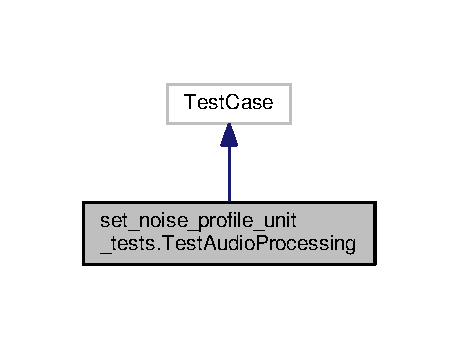
\includegraphics[width=220pt]{classset__noise__profile__unit__tests_1_1TestAudioProcessing__inherit__graph}
\end{center}
\end{figure}


Collaboration diagram for set\-\_\-noise\-\_\-profile\-\_\-unit\-\_\-tests.\-Test\-Audio\-Processing\-:
\nopagebreak
\begin{figure}[H]
\begin{center}
\leavevmode
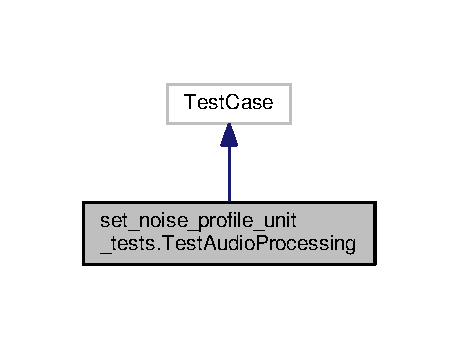
\includegraphics[width=220pt]{classset__noise__profile__unit__tests_1_1TestAudioProcessing__coll__graph}
\end{center}
\end{figure}
\subsection*{Public Member Functions}
\begin{DoxyCompactItemize}
\item 
def \hyperlink{classset__noise__profile__unit__tests_1_1TestAudioProcessing_aa7eba721c2137e085d71fd1126929876}{set\-Up}
\item 
def \hyperlink{classset__noise__profile__unit__tests_1_1TestAudioProcessing_abfbcf658ea73b62d4b94016a778515f4}{tear\-Down}
\item 
def \hyperlink{classset__noise__profile__unit__tests_1_1TestAudioProcessing_a6293aff3a1f71fdcd51393ae57948a32}{test\-\_\-no\-\_\-silence\-\_\-file}
\item 
def \hyperlink{classset__noise__profile__unit__tests_1_1TestAudioProcessing_aae66bc9e72046243dd4a1cbd43a5dae5}{test\-\_\-ogg}
\item 
def \hyperlink{classset__noise__profile__unit__tests_1_1TestAudioProcessing_a9e4063805c8545ba621b7e09fba15c60}{test\-\_\-ogg\-\_\-with\-\_\-wav\-\_\-1\-\_\-ch\-\_\-type}
\item 
def \hyperlink{classset__noise__profile__unit__tests_1_1TestAudioProcessing_a5f997de787a67b81ec5e33b8b2d23615}{test\-\_\-ogg\-\_\-with\-\_\-wav\-\_\-4\-\_\-ch\-\_\-type}
\item 
def \hyperlink{classset__noise__profile__unit__tests_1_1TestAudioProcessing_a7b2dbff468be7478d9a1386a3bab6ac9}{test\-\_\-wav\-\_\-1\-\_\-ch}
\item 
def \hyperlink{classset__noise__profile__unit__tests_1_1TestAudioProcessing_a72be9bf00b4fbe3248e71b8c17201f02}{test\-\_\-wav\-\_\-1\-\_\-ch\-\_\-with\-\_\-ogg\-\_\-type}
\item 
def \hyperlink{classset__noise__profile__unit__tests_1_1TestAudioProcessing_a21bb7d6856ed95d70e3e6c5e3d7cd294}{test\-\_\-wav\-\_\-1\-\_\-ch\-\_\-with\-\_\-wav\-\_\-4\-\_\-ch\-\_\-type}
\item 
def \hyperlink{classset__noise__profile__unit__tests_1_1TestAudioProcessing_ae81e405165fb08eafcf2d24e524ba6d6}{test\-\_\-wav\-\_\-4\-\_\-ch}
\item 
def \hyperlink{classset__noise__profile__unit__tests_1_1TestAudioProcessing_a7b76d128b1f1ff7e84bdbbed37deffe7}{test\-\_\-wav\-\_\-4\-\_\-ch\-\_\-with\-\_\-ogg\-\_\-type}
\item 
def \hyperlink{classset__noise__profile__unit__tests_1_1TestAudioProcessing_a8fcca5d1c4f97bb316bbc10b252585d9}{test\-\_\-wav\-\_\-4\-\_\-ch\-\_\-with\-\_\-wav\-\_\-1\-\_\-ch\-\_\-type}
\item 
def \hyperlink{classset__noise__profile__unit__tests_1_1TestAudioProcessing_acd1924ca4d59275d8f8841fe43d79f67}{test\-\_\-wav\-\_\-6\-\_\-ch}
\end{DoxyCompactItemize}
\subsection*{Public Attributes}
\begin{DoxyCompactItemize}
\item 
\hyperlink{classset__noise__profile__unit__tests_1_1TestAudioProcessing_af90ba77fd1a22f2ef9bf1150ed7755bc}{auxiliary\-\_\-files\-\_\-url}
\item 
\hyperlink{classset__noise__profile__unit__tests_1_1TestAudioProcessing_aa8588c51c5c1fc980988138c0ee6f8c8}{module}
\item 
\hyperlink{classset__noise__profile__unit__tests_1_1TestAudioProcessing_a9cee1cae109530cd693c9e859b33a7f8}{rospack}
\end{DoxyCompactItemize}


\subsection{Detailed Description}


Definition at line 31 of file set\-\_\-noise\-\_\-profile\-\_\-unit\-\_\-tests.\-py.



\subsection{Member Function Documentation}
\hypertarget{classset__noise__profile__unit__tests_1_1TestAudioProcessing_aa7eba721c2137e085d71fd1126929876}{\index{set\-\_\-noise\-\_\-profile\-\_\-unit\-\_\-tests\-::\-Test\-Audio\-Processing@{set\-\_\-noise\-\_\-profile\-\_\-unit\-\_\-tests\-::\-Test\-Audio\-Processing}!set\-Up@{set\-Up}}
\index{set\-Up@{set\-Up}!set_noise_profile_unit_tests::TestAudioProcessing@{set\-\_\-noise\-\_\-profile\-\_\-unit\-\_\-tests\-::\-Test\-Audio\-Processing}}
\subsubsection[{set\-Up}]{\setlength{\rightskip}{0pt plus 5cm}def set\-\_\-noise\-\_\-profile\-\_\-unit\-\_\-tests.\-Test\-Audio\-Processing.\-set\-Up (
\begin{DoxyParamCaption}
\item[{}]{self}
\end{DoxyParamCaption}
)}}\label{classset__noise__profile__unit__tests_1_1TestAudioProcessing_aa7eba721c2137e085d71fd1126929876}


Definition at line 32 of file set\-\_\-noise\-\_\-profile\-\_\-unit\-\_\-tests.\-py.

\hypertarget{classset__noise__profile__unit__tests_1_1TestAudioProcessing_abfbcf658ea73b62d4b94016a778515f4}{\index{set\-\_\-noise\-\_\-profile\-\_\-unit\-\_\-tests\-::\-Test\-Audio\-Processing@{set\-\_\-noise\-\_\-profile\-\_\-unit\-\_\-tests\-::\-Test\-Audio\-Processing}!tear\-Down@{tear\-Down}}
\index{tear\-Down@{tear\-Down}!set_noise_profile_unit_tests::TestAudioProcessing@{set\-\_\-noise\-\_\-profile\-\_\-unit\-\_\-tests\-::\-Test\-Audio\-Processing}}
\subsubsection[{tear\-Down}]{\setlength{\rightskip}{0pt plus 5cm}def set\-\_\-noise\-\_\-profile\-\_\-unit\-\_\-tests.\-Test\-Audio\-Processing.\-tear\-Down (
\begin{DoxyParamCaption}
\item[{}]{self}
\end{DoxyParamCaption}
)}}\label{classset__noise__profile__unit__tests_1_1TestAudioProcessing_abfbcf658ea73b62d4b94016a778515f4}


Definition at line 38 of file set\-\_\-noise\-\_\-profile\-\_\-unit\-\_\-tests.\-py.

\hypertarget{classset__noise__profile__unit__tests_1_1TestAudioProcessing_a6293aff3a1f71fdcd51393ae57948a32}{\index{set\-\_\-noise\-\_\-profile\-\_\-unit\-\_\-tests\-::\-Test\-Audio\-Processing@{set\-\_\-noise\-\_\-profile\-\_\-unit\-\_\-tests\-::\-Test\-Audio\-Processing}!test\-\_\-no\-\_\-silence\-\_\-file@{test\-\_\-no\-\_\-silence\-\_\-file}}
\index{test\-\_\-no\-\_\-silence\-\_\-file@{test\-\_\-no\-\_\-silence\-\_\-file}!set_noise_profile_unit_tests::TestAudioProcessing@{set\-\_\-noise\-\_\-profile\-\_\-unit\-\_\-tests\-::\-Test\-Audio\-Processing}}
\subsubsection[{test\-\_\-no\-\_\-silence\-\_\-file}]{\setlength{\rightskip}{0pt plus 5cm}def set\-\_\-noise\-\_\-profile\-\_\-unit\-\_\-tests.\-Test\-Audio\-Processing.\-test\-\_\-no\-\_\-silence\-\_\-file (
\begin{DoxyParamCaption}
\item[{}]{self}
\end{DoxyParamCaption}
)}}\label{classset__noise__profile__unit__tests_1_1TestAudioProcessing_a6293aff3a1f71fdcd51393ae57948a32}


Definition at line 92 of file set\-\_\-noise\-\_\-profile\-\_\-unit\-\_\-tests.\-py.

\hypertarget{classset__noise__profile__unit__tests_1_1TestAudioProcessing_aae66bc9e72046243dd4a1cbd43a5dae5}{\index{set\-\_\-noise\-\_\-profile\-\_\-unit\-\_\-tests\-::\-Test\-Audio\-Processing@{set\-\_\-noise\-\_\-profile\-\_\-unit\-\_\-tests\-::\-Test\-Audio\-Processing}!test\-\_\-ogg@{test\-\_\-ogg}}
\index{test\-\_\-ogg@{test\-\_\-ogg}!set_noise_profile_unit_tests::TestAudioProcessing@{set\-\_\-noise\-\_\-profile\-\_\-unit\-\_\-tests\-::\-Test\-Audio\-Processing}}
\subsubsection[{test\-\_\-ogg}]{\setlength{\rightskip}{0pt plus 5cm}def set\-\_\-noise\-\_\-profile\-\_\-unit\-\_\-tests.\-Test\-Audio\-Processing.\-test\-\_\-ogg (
\begin{DoxyParamCaption}
\item[{}]{self}
\end{DoxyParamCaption}
)}}\label{classset__noise__profile__unit__tests_1_1TestAudioProcessing_aae66bc9e72046243dd4a1cbd43a5dae5}


Definition at line 42 of file set\-\_\-noise\-\_\-profile\-\_\-unit\-\_\-tests.\-py.

\hypertarget{classset__noise__profile__unit__tests_1_1TestAudioProcessing_a9e4063805c8545ba621b7e09fba15c60}{\index{set\-\_\-noise\-\_\-profile\-\_\-unit\-\_\-tests\-::\-Test\-Audio\-Processing@{set\-\_\-noise\-\_\-profile\-\_\-unit\-\_\-tests\-::\-Test\-Audio\-Processing}!test\-\_\-ogg\-\_\-with\-\_\-wav\-\_\-1\-\_\-ch\-\_\-type@{test\-\_\-ogg\-\_\-with\-\_\-wav\-\_\-1\-\_\-ch\-\_\-type}}
\index{test\-\_\-ogg\-\_\-with\-\_\-wav\-\_\-1\-\_\-ch\-\_\-type@{test\-\_\-ogg\-\_\-with\-\_\-wav\-\_\-1\-\_\-ch\-\_\-type}!set_noise_profile_unit_tests::TestAudioProcessing@{set\-\_\-noise\-\_\-profile\-\_\-unit\-\_\-tests\-::\-Test\-Audio\-Processing}}
\subsubsection[{test\-\_\-ogg\-\_\-with\-\_\-wav\-\_\-1\-\_\-ch\-\_\-type}]{\setlength{\rightskip}{0pt plus 5cm}def set\-\_\-noise\-\_\-profile\-\_\-unit\-\_\-tests.\-Test\-Audio\-Processing.\-test\-\_\-ogg\-\_\-with\-\_\-wav\-\_\-1\-\_\-ch\-\_\-type (
\begin{DoxyParamCaption}
\item[{}]{self}
\end{DoxyParamCaption}
)}}\label{classset__noise__profile__unit__tests_1_1TestAudioProcessing_a9e4063805c8545ba621b7e09fba15c60}


Definition at line 127 of file set\-\_\-noise\-\_\-profile\-\_\-unit\-\_\-tests.\-py.

\hypertarget{classset__noise__profile__unit__tests_1_1TestAudioProcessing_a5f997de787a67b81ec5e33b8b2d23615}{\index{set\-\_\-noise\-\_\-profile\-\_\-unit\-\_\-tests\-::\-Test\-Audio\-Processing@{set\-\_\-noise\-\_\-profile\-\_\-unit\-\_\-tests\-::\-Test\-Audio\-Processing}!test\-\_\-ogg\-\_\-with\-\_\-wav\-\_\-4\-\_\-ch\-\_\-type@{test\-\_\-ogg\-\_\-with\-\_\-wav\-\_\-4\-\_\-ch\-\_\-type}}
\index{test\-\_\-ogg\-\_\-with\-\_\-wav\-\_\-4\-\_\-ch\-\_\-type@{test\-\_\-ogg\-\_\-with\-\_\-wav\-\_\-4\-\_\-ch\-\_\-type}!set_noise_profile_unit_tests::TestAudioProcessing@{set\-\_\-noise\-\_\-profile\-\_\-unit\-\_\-tests\-::\-Test\-Audio\-Processing}}
\subsubsection[{test\-\_\-ogg\-\_\-with\-\_\-wav\-\_\-4\-\_\-ch\-\_\-type}]{\setlength{\rightskip}{0pt plus 5cm}def set\-\_\-noise\-\_\-profile\-\_\-unit\-\_\-tests.\-Test\-Audio\-Processing.\-test\-\_\-ogg\-\_\-with\-\_\-wav\-\_\-4\-\_\-ch\-\_\-type (
\begin{DoxyParamCaption}
\item[{}]{self}
\end{DoxyParamCaption}
)}}\label{classset__noise__profile__unit__tests_1_1TestAudioProcessing_a5f997de787a67b81ec5e33b8b2d23615}


Definition at line 134 of file set\-\_\-noise\-\_\-profile\-\_\-unit\-\_\-tests.\-py.

\hypertarget{classset__noise__profile__unit__tests_1_1TestAudioProcessing_a7b2dbff468be7478d9a1386a3bab6ac9}{\index{set\-\_\-noise\-\_\-profile\-\_\-unit\-\_\-tests\-::\-Test\-Audio\-Processing@{set\-\_\-noise\-\_\-profile\-\_\-unit\-\_\-tests\-::\-Test\-Audio\-Processing}!test\-\_\-wav\-\_\-1\-\_\-ch@{test\-\_\-wav\-\_\-1\-\_\-ch}}
\index{test\-\_\-wav\-\_\-1\-\_\-ch@{test\-\_\-wav\-\_\-1\-\_\-ch}!set_noise_profile_unit_tests::TestAudioProcessing@{set\-\_\-noise\-\_\-profile\-\_\-unit\-\_\-tests\-::\-Test\-Audio\-Processing}}
\subsubsection[{test\-\_\-wav\-\_\-1\-\_\-ch}]{\setlength{\rightskip}{0pt plus 5cm}def set\-\_\-noise\-\_\-profile\-\_\-unit\-\_\-tests.\-Test\-Audio\-Processing.\-test\-\_\-wav\-\_\-1\-\_\-ch (
\begin{DoxyParamCaption}
\item[{}]{self}
\end{DoxyParamCaption}
)}}\label{classset__noise__profile__unit__tests_1_1TestAudioProcessing_a7b2dbff468be7478d9a1386a3bab6ac9}


Definition at line 57 of file set\-\_\-noise\-\_\-profile\-\_\-unit\-\_\-tests.\-py.

\hypertarget{classset__noise__profile__unit__tests_1_1TestAudioProcessing_a72be9bf00b4fbe3248e71b8c17201f02}{\index{set\-\_\-noise\-\_\-profile\-\_\-unit\-\_\-tests\-::\-Test\-Audio\-Processing@{set\-\_\-noise\-\_\-profile\-\_\-unit\-\_\-tests\-::\-Test\-Audio\-Processing}!test\-\_\-wav\-\_\-1\-\_\-ch\-\_\-with\-\_\-ogg\-\_\-type@{test\-\_\-wav\-\_\-1\-\_\-ch\-\_\-with\-\_\-ogg\-\_\-type}}
\index{test\-\_\-wav\-\_\-1\-\_\-ch\-\_\-with\-\_\-ogg\-\_\-type@{test\-\_\-wav\-\_\-1\-\_\-ch\-\_\-with\-\_\-ogg\-\_\-type}!set_noise_profile_unit_tests::TestAudioProcessing@{set\-\_\-noise\-\_\-profile\-\_\-unit\-\_\-tests\-::\-Test\-Audio\-Processing}}
\subsubsection[{test\-\_\-wav\-\_\-1\-\_\-ch\-\_\-with\-\_\-ogg\-\_\-type}]{\setlength{\rightskip}{0pt plus 5cm}def set\-\_\-noise\-\_\-profile\-\_\-unit\-\_\-tests.\-Test\-Audio\-Processing.\-test\-\_\-wav\-\_\-1\-\_\-ch\-\_\-with\-\_\-ogg\-\_\-type (
\begin{DoxyParamCaption}
\item[{}]{self}
\end{DoxyParamCaption}
)}}\label{classset__noise__profile__unit__tests_1_1TestAudioProcessing_a72be9bf00b4fbe3248e71b8c17201f02}


Definition at line 99 of file set\-\_\-noise\-\_\-profile\-\_\-unit\-\_\-tests.\-py.

\hypertarget{classset__noise__profile__unit__tests_1_1TestAudioProcessing_a21bb7d6856ed95d70e3e6c5e3d7cd294}{\index{set\-\_\-noise\-\_\-profile\-\_\-unit\-\_\-tests\-::\-Test\-Audio\-Processing@{set\-\_\-noise\-\_\-profile\-\_\-unit\-\_\-tests\-::\-Test\-Audio\-Processing}!test\-\_\-wav\-\_\-1\-\_\-ch\-\_\-with\-\_\-wav\-\_\-4\-\_\-ch\-\_\-type@{test\-\_\-wav\-\_\-1\-\_\-ch\-\_\-with\-\_\-wav\-\_\-4\-\_\-ch\-\_\-type}}
\index{test\-\_\-wav\-\_\-1\-\_\-ch\-\_\-with\-\_\-wav\-\_\-4\-\_\-ch\-\_\-type@{test\-\_\-wav\-\_\-1\-\_\-ch\-\_\-with\-\_\-wav\-\_\-4\-\_\-ch\-\_\-type}!set_noise_profile_unit_tests::TestAudioProcessing@{set\-\_\-noise\-\_\-profile\-\_\-unit\-\_\-tests\-::\-Test\-Audio\-Processing}}
\subsubsection[{test\-\_\-wav\-\_\-1\-\_\-ch\-\_\-with\-\_\-wav\-\_\-4\-\_\-ch\-\_\-type}]{\setlength{\rightskip}{0pt plus 5cm}def set\-\_\-noise\-\_\-profile\-\_\-unit\-\_\-tests.\-Test\-Audio\-Processing.\-test\-\_\-wav\-\_\-1\-\_\-ch\-\_\-with\-\_\-wav\-\_\-4\-\_\-ch\-\_\-type (
\begin{DoxyParamCaption}
\item[{}]{self}
\end{DoxyParamCaption}
)}}\label{classset__noise__profile__unit__tests_1_1TestAudioProcessing_a21bb7d6856ed95d70e3e6c5e3d7cd294}


Definition at line 106 of file set\-\_\-noise\-\_\-profile\-\_\-unit\-\_\-tests.\-py.

\hypertarget{classset__noise__profile__unit__tests_1_1TestAudioProcessing_ae81e405165fb08eafcf2d24e524ba6d6}{\index{set\-\_\-noise\-\_\-profile\-\_\-unit\-\_\-tests\-::\-Test\-Audio\-Processing@{set\-\_\-noise\-\_\-profile\-\_\-unit\-\_\-tests\-::\-Test\-Audio\-Processing}!test\-\_\-wav\-\_\-4\-\_\-ch@{test\-\_\-wav\-\_\-4\-\_\-ch}}
\index{test\-\_\-wav\-\_\-4\-\_\-ch@{test\-\_\-wav\-\_\-4\-\_\-ch}!set_noise_profile_unit_tests::TestAudioProcessing@{set\-\_\-noise\-\_\-profile\-\_\-unit\-\_\-tests\-::\-Test\-Audio\-Processing}}
\subsubsection[{test\-\_\-wav\-\_\-4\-\_\-ch}]{\setlength{\rightskip}{0pt plus 5cm}def set\-\_\-noise\-\_\-profile\-\_\-unit\-\_\-tests.\-Test\-Audio\-Processing.\-test\-\_\-wav\-\_\-4\-\_\-ch (
\begin{DoxyParamCaption}
\item[{}]{self}
\end{DoxyParamCaption}
)}}\label{classset__noise__profile__unit__tests_1_1TestAudioProcessing_ae81e405165fb08eafcf2d24e524ba6d6}


Definition at line 71 of file set\-\_\-noise\-\_\-profile\-\_\-unit\-\_\-tests.\-py.

\hypertarget{classset__noise__profile__unit__tests_1_1TestAudioProcessing_a7b76d128b1f1ff7e84bdbbed37deffe7}{\index{set\-\_\-noise\-\_\-profile\-\_\-unit\-\_\-tests\-::\-Test\-Audio\-Processing@{set\-\_\-noise\-\_\-profile\-\_\-unit\-\_\-tests\-::\-Test\-Audio\-Processing}!test\-\_\-wav\-\_\-4\-\_\-ch\-\_\-with\-\_\-ogg\-\_\-type@{test\-\_\-wav\-\_\-4\-\_\-ch\-\_\-with\-\_\-ogg\-\_\-type}}
\index{test\-\_\-wav\-\_\-4\-\_\-ch\-\_\-with\-\_\-ogg\-\_\-type@{test\-\_\-wav\-\_\-4\-\_\-ch\-\_\-with\-\_\-ogg\-\_\-type}!set_noise_profile_unit_tests::TestAudioProcessing@{set\-\_\-noise\-\_\-profile\-\_\-unit\-\_\-tests\-::\-Test\-Audio\-Processing}}
\subsubsection[{test\-\_\-wav\-\_\-4\-\_\-ch\-\_\-with\-\_\-ogg\-\_\-type}]{\setlength{\rightskip}{0pt plus 5cm}def set\-\_\-noise\-\_\-profile\-\_\-unit\-\_\-tests.\-Test\-Audio\-Processing.\-test\-\_\-wav\-\_\-4\-\_\-ch\-\_\-with\-\_\-ogg\-\_\-type (
\begin{DoxyParamCaption}
\item[{}]{self}
\end{DoxyParamCaption}
)}}\label{classset__noise__profile__unit__tests_1_1TestAudioProcessing_a7b76d128b1f1ff7e84bdbbed37deffe7}


Definition at line 113 of file set\-\_\-noise\-\_\-profile\-\_\-unit\-\_\-tests.\-py.

\hypertarget{classset__noise__profile__unit__tests_1_1TestAudioProcessing_a8fcca5d1c4f97bb316bbc10b252585d9}{\index{set\-\_\-noise\-\_\-profile\-\_\-unit\-\_\-tests\-::\-Test\-Audio\-Processing@{set\-\_\-noise\-\_\-profile\-\_\-unit\-\_\-tests\-::\-Test\-Audio\-Processing}!test\-\_\-wav\-\_\-4\-\_\-ch\-\_\-with\-\_\-wav\-\_\-1\-\_\-ch\-\_\-type@{test\-\_\-wav\-\_\-4\-\_\-ch\-\_\-with\-\_\-wav\-\_\-1\-\_\-ch\-\_\-type}}
\index{test\-\_\-wav\-\_\-4\-\_\-ch\-\_\-with\-\_\-wav\-\_\-1\-\_\-ch\-\_\-type@{test\-\_\-wav\-\_\-4\-\_\-ch\-\_\-with\-\_\-wav\-\_\-1\-\_\-ch\-\_\-type}!set_noise_profile_unit_tests::TestAudioProcessing@{set\-\_\-noise\-\_\-profile\-\_\-unit\-\_\-tests\-::\-Test\-Audio\-Processing}}
\subsubsection[{test\-\_\-wav\-\_\-4\-\_\-ch\-\_\-with\-\_\-wav\-\_\-1\-\_\-ch\-\_\-type}]{\setlength{\rightskip}{0pt plus 5cm}def set\-\_\-noise\-\_\-profile\-\_\-unit\-\_\-tests.\-Test\-Audio\-Processing.\-test\-\_\-wav\-\_\-4\-\_\-ch\-\_\-with\-\_\-wav\-\_\-1\-\_\-ch\-\_\-type (
\begin{DoxyParamCaption}
\item[{}]{self}
\end{DoxyParamCaption}
)}}\label{classset__noise__profile__unit__tests_1_1TestAudioProcessing_a8fcca5d1c4f97bb316bbc10b252585d9}


Definition at line 120 of file set\-\_\-noise\-\_\-profile\-\_\-unit\-\_\-tests.\-py.

\hypertarget{classset__noise__profile__unit__tests_1_1TestAudioProcessing_acd1924ca4d59275d8f8841fe43d79f67}{\index{set\-\_\-noise\-\_\-profile\-\_\-unit\-\_\-tests\-::\-Test\-Audio\-Processing@{set\-\_\-noise\-\_\-profile\-\_\-unit\-\_\-tests\-::\-Test\-Audio\-Processing}!test\-\_\-wav\-\_\-6\-\_\-ch@{test\-\_\-wav\-\_\-6\-\_\-ch}}
\index{test\-\_\-wav\-\_\-6\-\_\-ch@{test\-\_\-wav\-\_\-6\-\_\-ch}!set_noise_profile_unit_tests::TestAudioProcessing@{set\-\_\-noise\-\_\-profile\-\_\-unit\-\_\-tests\-::\-Test\-Audio\-Processing}}
\subsubsection[{test\-\_\-wav\-\_\-6\-\_\-ch}]{\setlength{\rightskip}{0pt plus 5cm}def set\-\_\-noise\-\_\-profile\-\_\-unit\-\_\-tests.\-Test\-Audio\-Processing.\-test\-\_\-wav\-\_\-6\-\_\-ch (
\begin{DoxyParamCaption}
\item[{}]{self}
\end{DoxyParamCaption}
)}}\label{classset__noise__profile__unit__tests_1_1TestAudioProcessing_acd1924ca4d59275d8f8841fe43d79f67}


Definition at line 85 of file set\-\_\-noise\-\_\-profile\-\_\-unit\-\_\-tests.\-py.



\subsection{Member Data Documentation}
\hypertarget{classset__noise__profile__unit__tests_1_1TestAudioProcessing_af90ba77fd1a22f2ef9bf1150ed7755bc}{\index{set\-\_\-noise\-\_\-profile\-\_\-unit\-\_\-tests\-::\-Test\-Audio\-Processing@{set\-\_\-noise\-\_\-profile\-\_\-unit\-\_\-tests\-::\-Test\-Audio\-Processing}!auxiliary\-\_\-files\-\_\-url@{auxiliary\-\_\-files\-\_\-url}}
\index{auxiliary\-\_\-files\-\_\-url@{auxiliary\-\_\-files\-\_\-url}!set_noise_profile_unit_tests::TestAudioProcessing@{set\-\_\-noise\-\_\-profile\-\_\-unit\-\_\-tests\-::\-Test\-Audio\-Processing}}
\subsubsection[{auxiliary\-\_\-files\-\_\-url}]{\setlength{\rightskip}{0pt plus 5cm}set\-\_\-noise\-\_\-profile\-\_\-unit\-\_\-tests.\-Test\-Audio\-Processing.\-auxiliary\-\_\-files\-\_\-url}}\label{classset__noise__profile__unit__tests_1_1TestAudioProcessing_af90ba77fd1a22f2ef9bf1150ed7755bc}


Definition at line 34 of file set\-\_\-noise\-\_\-profile\-\_\-unit\-\_\-tests.\-py.

\hypertarget{classset__noise__profile__unit__tests_1_1TestAudioProcessing_aa8588c51c5c1fc980988138c0ee6f8c8}{\index{set\-\_\-noise\-\_\-profile\-\_\-unit\-\_\-tests\-::\-Test\-Audio\-Processing@{set\-\_\-noise\-\_\-profile\-\_\-unit\-\_\-tests\-::\-Test\-Audio\-Processing}!module@{module}}
\index{module@{module}!set_noise_profile_unit_tests::TestAudioProcessing@{set\-\_\-noise\-\_\-profile\-\_\-unit\-\_\-tests\-::\-Test\-Audio\-Processing}}
\subsubsection[{module}]{\setlength{\rightskip}{0pt plus 5cm}set\-\_\-noise\-\_\-profile\-\_\-unit\-\_\-tests.\-Test\-Audio\-Processing.\-module}}\label{classset__noise__profile__unit__tests_1_1TestAudioProcessing_aa8588c51c5c1fc980988138c0ee6f8c8}


Definition at line 36 of file set\-\_\-noise\-\_\-profile\-\_\-unit\-\_\-tests.\-py.

\hypertarget{classset__noise__profile__unit__tests_1_1TestAudioProcessing_a9cee1cae109530cd693c9e859b33a7f8}{\index{set\-\_\-noise\-\_\-profile\-\_\-unit\-\_\-tests\-::\-Test\-Audio\-Processing@{set\-\_\-noise\-\_\-profile\-\_\-unit\-\_\-tests\-::\-Test\-Audio\-Processing}!rospack@{rospack}}
\index{rospack@{rospack}!set_noise_profile_unit_tests::TestAudioProcessing@{set\-\_\-noise\-\_\-profile\-\_\-unit\-\_\-tests\-::\-Test\-Audio\-Processing}}
\subsubsection[{rospack}]{\setlength{\rightskip}{0pt plus 5cm}set\-\_\-noise\-\_\-profile\-\_\-unit\-\_\-tests.\-Test\-Audio\-Processing.\-rospack}}\label{classset__noise__profile__unit__tests_1_1TestAudioProcessing_a9cee1cae109530cd693c9e859b33a7f8}


Definition at line 40 of file set\-\_\-noise\-\_\-profile\-\_\-unit\-\_\-tests.\-py.



The documentation for this class was generated from the following file\-:\begin{DoxyCompactItemize}
\item 
/home/travis/rapp\-\_\-temp/rapp-\/platform/rapp\-\_\-audio\-\_\-processing/tests/unit/\hyperlink{set__noise__profile__unit__tests_8py}{set\-\_\-noise\-\_\-profile\-\_\-unit\-\_\-tests.\-py}\end{DoxyCompactItemize}

\hypertarget{classenergy__denoise__unit__tests_1_1TestAudioProcessing}{\section{energy\-\_\-denoise\-\_\-unit\-\_\-tests.\-Test\-Audio\-Processing Class Reference}
\label{classenergy__denoise__unit__tests_1_1TestAudioProcessing}\index{energy\-\_\-denoise\-\_\-unit\-\_\-tests.\-Test\-Audio\-Processing@{energy\-\_\-denoise\-\_\-unit\-\_\-tests.\-Test\-Audio\-Processing}}
}


Inheritance diagram for energy\-\_\-denoise\-\_\-unit\-\_\-tests.\-Test\-Audio\-Processing\-:


Collaboration diagram for energy\-\_\-denoise\-\_\-unit\-\_\-tests.\-Test\-Audio\-Processing\-:
\subsection*{Public Member Functions}
\begin{DoxyCompactItemize}
\item 
def \hyperlink{classenergy__denoise__unit__tests_1_1TestAudioProcessing_a44c374336e29472cc652b67ab0dada30}{set\-Up}
\item 
def \hyperlink{classenergy__denoise__unit__tests_1_1TestAudioProcessing_a55c6e949339b8570f70110a175ceec0f}{tear\-Down}
\item 
def \hyperlink{classenergy__denoise__unit__tests_1_1TestAudioProcessing_a811ed04be3321882fa8eb15be7762718}{test\-\_\-energy\-\_\-denois}
\item 
def \hyperlink{classenergy__denoise__unit__tests_1_1TestAudioProcessing_a0b6da8782f3e5ed188fae3be9a051616}{test\-\_\-not\-Existent\-File}
\end{DoxyCompactItemize}
\subsection*{Public Attributes}
\begin{DoxyCompactItemize}
\item 
\hyperlink{classenergy__denoise__unit__tests_1_1TestAudioProcessing_a90a81b0f2553ca8b64eb8b430ec0b61f}{auxiliary\-\_\-files\-\_\-url}
\item 
\hyperlink{classenergy__denoise__unit__tests_1_1TestAudioProcessing_acccf9990be3626520addd73fdbaaf4ea}{energy\-\_\-denoise\-\_\-module}
\item 
\hyperlink{classenergy__denoise__unit__tests_1_1TestAudioProcessing_a25b1514d4fd69a373b58def2b5c76719}{rospack}
\end{DoxyCompactItemize}


\subsection{Detailed Description}


Definition at line 33 of file energy\-\_\-denoise\-\_\-unit\-\_\-tests.\-py.



\subsection{Member Function Documentation}
\hypertarget{classenergy__denoise__unit__tests_1_1TestAudioProcessing_a44c374336e29472cc652b67ab0dada30}{\index{energy\-\_\-denoise\-\_\-unit\-\_\-tests\-::\-Test\-Audio\-Processing@{energy\-\_\-denoise\-\_\-unit\-\_\-tests\-::\-Test\-Audio\-Processing}!set\-Up@{set\-Up}}
\index{set\-Up@{set\-Up}!energy_denoise_unit_tests::TestAudioProcessing@{energy\-\_\-denoise\-\_\-unit\-\_\-tests\-::\-Test\-Audio\-Processing}}
\subsubsection[{set\-Up}]{\setlength{\rightskip}{0pt plus 5cm}def energy\-\_\-denoise\-\_\-unit\-\_\-tests.\-Test\-Audio\-Processing.\-set\-Up (
\begin{DoxyParamCaption}
\item[{}]{self}
\end{DoxyParamCaption}
)}}\label{classenergy__denoise__unit__tests_1_1TestAudioProcessing_a44c374336e29472cc652b67ab0dada30}


Definition at line 34 of file energy\-\_\-denoise\-\_\-unit\-\_\-tests.\-py.

\hypertarget{classenergy__denoise__unit__tests_1_1TestAudioProcessing_a55c6e949339b8570f70110a175ceec0f}{\index{energy\-\_\-denoise\-\_\-unit\-\_\-tests\-::\-Test\-Audio\-Processing@{energy\-\_\-denoise\-\_\-unit\-\_\-tests\-::\-Test\-Audio\-Processing}!tear\-Down@{tear\-Down}}
\index{tear\-Down@{tear\-Down}!energy_denoise_unit_tests::TestAudioProcessing@{energy\-\_\-denoise\-\_\-unit\-\_\-tests\-::\-Test\-Audio\-Processing}}
\subsubsection[{tear\-Down}]{\setlength{\rightskip}{0pt plus 5cm}def energy\-\_\-denoise\-\_\-unit\-\_\-tests.\-Test\-Audio\-Processing.\-tear\-Down (
\begin{DoxyParamCaption}
\item[{}]{self}
\end{DoxyParamCaption}
)}}\label{classenergy__denoise__unit__tests_1_1TestAudioProcessing_a55c6e949339b8570f70110a175ceec0f}


Definition at line 40 of file energy\-\_\-denoise\-\_\-unit\-\_\-tests.\-py.

\hypertarget{classenergy__denoise__unit__tests_1_1TestAudioProcessing_a811ed04be3321882fa8eb15be7762718}{\index{energy\-\_\-denoise\-\_\-unit\-\_\-tests\-::\-Test\-Audio\-Processing@{energy\-\_\-denoise\-\_\-unit\-\_\-tests\-::\-Test\-Audio\-Processing}!test\-\_\-energy\-\_\-denois@{test\-\_\-energy\-\_\-denois}}
\index{test\-\_\-energy\-\_\-denois@{test\-\_\-energy\-\_\-denois}!energy_denoise_unit_tests::TestAudioProcessing@{energy\-\_\-denoise\-\_\-unit\-\_\-tests\-::\-Test\-Audio\-Processing}}
\subsubsection[{test\-\_\-energy\-\_\-denois}]{\setlength{\rightskip}{0pt plus 5cm}def energy\-\_\-denoise\-\_\-unit\-\_\-tests.\-Test\-Audio\-Processing.\-test\-\_\-energy\-\_\-denois (
\begin{DoxyParamCaption}
\item[{}]{self}
\end{DoxyParamCaption}
)}}\label{classenergy__denoise__unit__tests_1_1TestAudioProcessing_a811ed04be3321882fa8eb15be7762718}


Definition at line 44 of file energy\-\_\-denoise\-\_\-unit\-\_\-tests.\-py.

\hypertarget{classenergy__denoise__unit__tests_1_1TestAudioProcessing_a0b6da8782f3e5ed188fae3be9a051616}{\index{energy\-\_\-denoise\-\_\-unit\-\_\-tests\-::\-Test\-Audio\-Processing@{energy\-\_\-denoise\-\_\-unit\-\_\-tests\-::\-Test\-Audio\-Processing}!test\-\_\-not\-Existent\-File@{test\-\_\-not\-Existent\-File}}
\index{test\-\_\-not\-Existent\-File@{test\-\_\-not\-Existent\-File}!energy_denoise_unit_tests::TestAudioProcessing@{energy\-\_\-denoise\-\_\-unit\-\_\-tests\-::\-Test\-Audio\-Processing}}
\subsubsection[{test\-\_\-not\-Existent\-File}]{\setlength{\rightskip}{0pt plus 5cm}def energy\-\_\-denoise\-\_\-unit\-\_\-tests.\-Test\-Audio\-Processing.\-test\-\_\-not\-Existent\-File (
\begin{DoxyParamCaption}
\item[{}]{self}
\end{DoxyParamCaption}
)}}\label{classenergy__denoise__unit__tests_1_1TestAudioProcessing_a0b6da8782f3e5ed188fae3be9a051616}


Definition at line 72 of file energy\-\_\-denoise\-\_\-unit\-\_\-tests.\-py.



\subsection{Member Data Documentation}
\hypertarget{classenergy__denoise__unit__tests_1_1TestAudioProcessing_a90a81b0f2553ca8b64eb8b430ec0b61f}{\index{energy\-\_\-denoise\-\_\-unit\-\_\-tests\-::\-Test\-Audio\-Processing@{energy\-\_\-denoise\-\_\-unit\-\_\-tests\-::\-Test\-Audio\-Processing}!auxiliary\-\_\-files\-\_\-url@{auxiliary\-\_\-files\-\_\-url}}
\index{auxiliary\-\_\-files\-\_\-url@{auxiliary\-\_\-files\-\_\-url}!energy_denoise_unit_tests::TestAudioProcessing@{energy\-\_\-denoise\-\_\-unit\-\_\-tests\-::\-Test\-Audio\-Processing}}
\subsubsection[{auxiliary\-\_\-files\-\_\-url}]{\setlength{\rightskip}{0pt plus 5cm}energy\-\_\-denoise\-\_\-unit\-\_\-tests.\-Test\-Audio\-Processing.\-auxiliary\-\_\-files\-\_\-url}}\label{classenergy__denoise__unit__tests_1_1TestAudioProcessing_a90a81b0f2553ca8b64eb8b430ec0b61f}


Definition at line 36 of file energy\-\_\-denoise\-\_\-unit\-\_\-tests.\-py.

\hypertarget{classenergy__denoise__unit__tests_1_1TestAudioProcessing_acccf9990be3626520addd73fdbaaf4ea}{\index{energy\-\_\-denoise\-\_\-unit\-\_\-tests\-::\-Test\-Audio\-Processing@{energy\-\_\-denoise\-\_\-unit\-\_\-tests\-::\-Test\-Audio\-Processing}!energy\-\_\-denoise\-\_\-module@{energy\-\_\-denoise\-\_\-module}}
\index{energy\-\_\-denoise\-\_\-module@{energy\-\_\-denoise\-\_\-module}!energy_denoise_unit_tests::TestAudioProcessing@{energy\-\_\-denoise\-\_\-unit\-\_\-tests\-::\-Test\-Audio\-Processing}}
\subsubsection[{energy\-\_\-denoise\-\_\-module}]{\setlength{\rightskip}{0pt plus 5cm}energy\-\_\-denoise\-\_\-unit\-\_\-tests.\-Test\-Audio\-Processing.\-energy\-\_\-denoise\-\_\-module}}\label{classenergy__denoise__unit__tests_1_1TestAudioProcessing_acccf9990be3626520addd73fdbaaf4ea}


Definition at line 38 of file energy\-\_\-denoise\-\_\-unit\-\_\-tests.\-py.

\hypertarget{classenergy__denoise__unit__tests_1_1TestAudioProcessing_a25b1514d4fd69a373b58def2b5c76719}{\index{energy\-\_\-denoise\-\_\-unit\-\_\-tests\-::\-Test\-Audio\-Processing@{energy\-\_\-denoise\-\_\-unit\-\_\-tests\-::\-Test\-Audio\-Processing}!rospack@{rospack}}
\index{rospack@{rospack}!energy_denoise_unit_tests::TestAudioProcessing@{energy\-\_\-denoise\-\_\-unit\-\_\-tests\-::\-Test\-Audio\-Processing}}
\subsubsection[{rospack}]{\setlength{\rightskip}{0pt plus 5cm}energy\-\_\-denoise\-\_\-unit\-\_\-tests.\-Test\-Audio\-Processing.\-rospack}}\label{classenergy__denoise__unit__tests_1_1TestAudioProcessing_a25b1514d4fd69a373b58def2b5c76719}


Definition at line 42 of file energy\-\_\-denoise\-\_\-unit\-\_\-tests.\-py.



The documentation for this class was generated from the following file\-:\begin{DoxyCompactItemize}
\item 
/home/travis/rapp\-\_\-temp/rapp-\/platform/rapp\-\_\-audio\-\_\-processing/tests/unit/\hyperlink{energy__denoise__unit__tests_8py}{energy\-\_\-denoise\-\_\-unit\-\_\-tests.\-py}\end{DoxyCompactItemize}

\hypertarget{classdetect__silence__unit__tests_1_1TestAudioProcessing}{\section{detect\-\_\-silence\-\_\-unit\-\_\-tests.\-Test\-Audio\-Processing Class Reference}
\label{classdetect__silence__unit__tests_1_1TestAudioProcessing}\index{detect\-\_\-silence\-\_\-unit\-\_\-tests.\-Test\-Audio\-Processing@{detect\-\_\-silence\-\_\-unit\-\_\-tests.\-Test\-Audio\-Processing}}
}


Inheritance diagram for detect\-\_\-silence\-\_\-unit\-\_\-tests.\-Test\-Audio\-Processing\-:
\nopagebreak
\begin{figure}[H]
\begin{center}
\leavevmode
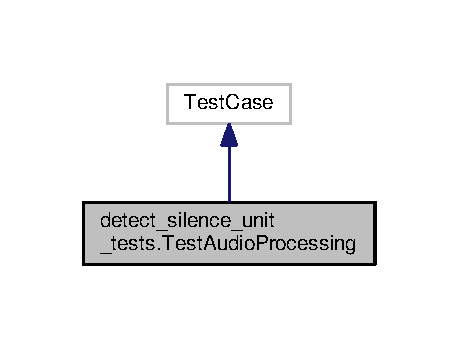
\includegraphics[width=220pt]{classdetect__silence__unit__tests_1_1TestAudioProcessing__inherit__graph}
\end{center}
\end{figure}


Collaboration diagram for detect\-\_\-silence\-\_\-unit\-\_\-tests.\-Test\-Audio\-Processing\-:
\nopagebreak
\begin{figure}[H]
\begin{center}
\leavevmode
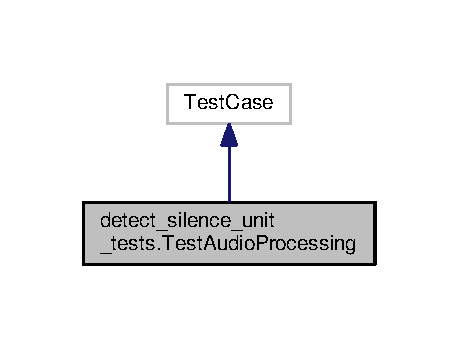
\includegraphics[width=220pt]{classdetect__silence__unit__tests_1_1TestAudioProcessing__coll__graph}
\end{center}
\end{figure}
\subsection*{Public Member Functions}
\begin{DoxyCompactItemize}
\item 
def \hyperlink{classdetect__silence__unit__tests_1_1TestAudioProcessing_a58df9540e3c490ad3060290a1f589714}{set\-Up}
\item 
def \hyperlink{classdetect__silence__unit__tests_1_1TestAudioProcessing_a04d23b9397b02367663ed9baca6c6860}{tear\-Down}
\item 
def \hyperlink{classdetect__silence__unit__tests_1_1TestAudioProcessing_a32cc654195575a3036122a1902dc612b}{test\-\_\-no\-Silence}
\item 
def \hyperlink{classdetect__silence__unit__tests_1_1TestAudioProcessing_acfd75c9a5d2b40194db63e2722870d20}{test\-\_\-not\-Existent\-File}
\item 
def \hyperlink{classdetect__silence__unit__tests_1_1TestAudioProcessing_a77b1ac9c346d4b12b4beed73d546acff}{test\-\_\-silence}
\end{DoxyCompactItemize}
\subsection*{Public Attributes}
\begin{DoxyCompactItemize}
\item 
\hyperlink{classdetect__silence__unit__tests_1_1TestAudioProcessing_a7c1bc7c6a2cca72c00260613a7c20bec}{auxiliary\-\_\-files\-\_\-url}
\item 
\hyperlink{classdetect__silence__unit__tests_1_1TestAudioProcessing_a091f6edd6c581d6bfb165a2aca2fd170}{detect\-\_\-silence\-\_\-module}
\item 
\hyperlink{classdetect__silence__unit__tests_1_1TestAudioProcessing_a484d0d9f66b7ff88516f206070db6afb}{rospack}
\end{DoxyCompactItemize}


\subsection{Detailed Description}


Definition at line 31 of file detect\-\_\-silence\-\_\-unit\-\_\-tests.\-py.



\subsection{Member Function Documentation}
\hypertarget{classdetect__silence__unit__tests_1_1TestAudioProcessing_a58df9540e3c490ad3060290a1f589714}{\index{detect\-\_\-silence\-\_\-unit\-\_\-tests\-::\-Test\-Audio\-Processing@{detect\-\_\-silence\-\_\-unit\-\_\-tests\-::\-Test\-Audio\-Processing}!set\-Up@{set\-Up}}
\index{set\-Up@{set\-Up}!detect_silence_unit_tests::TestAudioProcessing@{detect\-\_\-silence\-\_\-unit\-\_\-tests\-::\-Test\-Audio\-Processing}}
\subsubsection[{set\-Up}]{\setlength{\rightskip}{0pt plus 5cm}def detect\-\_\-silence\-\_\-unit\-\_\-tests.\-Test\-Audio\-Processing.\-set\-Up (
\begin{DoxyParamCaption}
\item[{}]{self}
\end{DoxyParamCaption}
)}}\label{classdetect__silence__unit__tests_1_1TestAudioProcessing_a58df9540e3c490ad3060290a1f589714}


Definition at line 32 of file detect\-\_\-silence\-\_\-unit\-\_\-tests.\-py.

\hypertarget{classdetect__silence__unit__tests_1_1TestAudioProcessing_a04d23b9397b02367663ed9baca6c6860}{\index{detect\-\_\-silence\-\_\-unit\-\_\-tests\-::\-Test\-Audio\-Processing@{detect\-\_\-silence\-\_\-unit\-\_\-tests\-::\-Test\-Audio\-Processing}!tear\-Down@{tear\-Down}}
\index{tear\-Down@{tear\-Down}!detect_silence_unit_tests::TestAudioProcessing@{detect\-\_\-silence\-\_\-unit\-\_\-tests\-::\-Test\-Audio\-Processing}}
\subsubsection[{tear\-Down}]{\setlength{\rightskip}{0pt plus 5cm}def detect\-\_\-silence\-\_\-unit\-\_\-tests.\-Test\-Audio\-Processing.\-tear\-Down (
\begin{DoxyParamCaption}
\item[{}]{self}
\end{DoxyParamCaption}
)}}\label{classdetect__silence__unit__tests_1_1TestAudioProcessing_a04d23b9397b02367663ed9baca6c6860}


Definition at line 38 of file detect\-\_\-silence\-\_\-unit\-\_\-tests.\-py.

\hypertarget{classdetect__silence__unit__tests_1_1TestAudioProcessing_a32cc654195575a3036122a1902dc612b}{\index{detect\-\_\-silence\-\_\-unit\-\_\-tests\-::\-Test\-Audio\-Processing@{detect\-\_\-silence\-\_\-unit\-\_\-tests\-::\-Test\-Audio\-Processing}!test\-\_\-no\-Silence@{test\-\_\-no\-Silence}}
\index{test\-\_\-no\-Silence@{test\-\_\-no\-Silence}!detect_silence_unit_tests::TestAudioProcessing@{detect\-\_\-silence\-\_\-unit\-\_\-tests\-::\-Test\-Audio\-Processing}}
\subsubsection[{test\-\_\-no\-Silence}]{\setlength{\rightskip}{0pt plus 5cm}def detect\-\_\-silence\-\_\-unit\-\_\-tests.\-Test\-Audio\-Processing.\-test\-\_\-no\-Silence (
\begin{DoxyParamCaption}
\item[{}]{self}
\end{DoxyParamCaption}
)}}\label{classdetect__silence__unit__tests_1_1TestAudioProcessing_a32cc654195575a3036122a1902dc612b}


Definition at line 47 of file detect\-\_\-silence\-\_\-unit\-\_\-tests.\-py.

\hypertarget{classdetect__silence__unit__tests_1_1TestAudioProcessing_acfd75c9a5d2b40194db63e2722870d20}{\index{detect\-\_\-silence\-\_\-unit\-\_\-tests\-::\-Test\-Audio\-Processing@{detect\-\_\-silence\-\_\-unit\-\_\-tests\-::\-Test\-Audio\-Processing}!test\-\_\-not\-Existent\-File@{test\-\_\-not\-Existent\-File}}
\index{test\-\_\-not\-Existent\-File@{test\-\_\-not\-Existent\-File}!detect_silence_unit_tests::TestAudioProcessing@{detect\-\_\-silence\-\_\-unit\-\_\-tests\-::\-Test\-Audio\-Processing}}
\subsubsection[{test\-\_\-not\-Existent\-File}]{\setlength{\rightskip}{0pt plus 5cm}def detect\-\_\-silence\-\_\-unit\-\_\-tests.\-Test\-Audio\-Processing.\-test\-\_\-not\-Existent\-File (
\begin{DoxyParamCaption}
\item[{}]{self}
\end{DoxyParamCaption}
)}}\label{classdetect__silence__unit__tests_1_1TestAudioProcessing_acfd75c9a5d2b40194db63e2722870d20}


Definition at line 52 of file detect\-\_\-silence\-\_\-unit\-\_\-tests.\-py.

\hypertarget{classdetect__silence__unit__tests_1_1TestAudioProcessing_a77b1ac9c346d4b12b4beed73d546acff}{\index{detect\-\_\-silence\-\_\-unit\-\_\-tests\-::\-Test\-Audio\-Processing@{detect\-\_\-silence\-\_\-unit\-\_\-tests\-::\-Test\-Audio\-Processing}!test\-\_\-silence@{test\-\_\-silence}}
\index{test\-\_\-silence@{test\-\_\-silence}!detect_silence_unit_tests::TestAudioProcessing@{detect\-\_\-silence\-\_\-unit\-\_\-tests\-::\-Test\-Audio\-Processing}}
\subsubsection[{test\-\_\-silence}]{\setlength{\rightskip}{0pt plus 5cm}def detect\-\_\-silence\-\_\-unit\-\_\-tests.\-Test\-Audio\-Processing.\-test\-\_\-silence (
\begin{DoxyParamCaption}
\item[{}]{self}
\end{DoxyParamCaption}
)}}\label{classdetect__silence__unit__tests_1_1TestAudioProcessing_a77b1ac9c346d4b12b4beed73d546acff}


Definition at line 42 of file detect\-\_\-silence\-\_\-unit\-\_\-tests.\-py.



\subsection{Member Data Documentation}
\hypertarget{classdetect__silence__unit__tests_1_1TestAudioProcessing_a7c1bc7c6a2cca72c00260613a7c20bec}{\index{detect\-\_\-silence\-\_\-unit\-\_\-tests\-::\-Test\-Audio\-Processing@{detect\-\_\-silence\-\_\-unit\-\_\-tests\-::\-Test\-Audio\-Processing}!auxiliary\-\_\-files\-\_\-url@{auxiliary\-\_\-files\-\_\-url}}
\index{auxiliary\-\_\-files\-\_\-url@{auxiliary\-\_\-files\-\_\-url}!detect_silence_unit_tests::TestAudioProcessing@{detect\-\_\-silence\-\_\-unit\-\_\-tests\-::\-Test\-Audio\-Processing}}
\subsubsection[{auxiliary\-\_\-files\-\_\-url}]{\setlength{\rightskip}{0pt plus 5cm}detect\-\_\-silence\-\_\-unit\-\_\-tests.\-Test\-Audio\-Processing.\-auxiliary\-\_\-files\-\_\-url}}\label{classdetect__silence__unit__tests_1_1TestAudioProcessing_a7c1bc7c6a2cca72c00260613a7c20bec}


Definition at line 34 of file detect\-\_\-silence\-\_\-unit\-\_\-tests.\-py.

\hypertarget{classdetect__silence__unit__tests_1_1TestAudioProcessing_a091f6edd6c581d6bfb165a2aca2fd170}{\index{detect\-\_\-silence\-\_\-unit\-\_\-tests\-::\-Test\-Audio\-Processing@{detect\-\_\-silence\-\_\-unit\-\_\-tests\-::\-Test\-Audio\-Processing}!detect\-\_\-silence\-\_\-module@{detect\-\_\-silence\-\_\-module}}
\index{detect\-\_\-silence\-\_\-module@{detect\-\_\-silence\-\_\-module}!detect_silence_unit_tests::TestAudioProcessing@{detect\-\_\-silence\-\_\-unit\-\_\-tests\-::\-Test\-Audio\-Processing}}
\subsubsection[{detect\-\_\-silence\-\_\-module}]{\setlength{\rightskip}{0pt plus 5cm}detect\-\_\-silence\-\_\-unit\-\_\-tests.\-Test\-Audio\-Processing.\-detect\-\_\-silence\-\_\-module}}\label{classdetect__silence__unit__tests_1_1TestAudioProcessing_a091f6edd6c581d6bfb165a2aca2fd170}


Definition at line 36 of file detect\-\_\-silence\-\_\-unit\-\_\-tests.\-py.

\hypertarget{classdetect__silence__unit__tests_1_1TestAudioProcessing_a484d0d9f66b7ff88516f206070db6afb}{\index{detect\-\_\-silence\-\_\-unit\-\_\-tests\-::\-Test\-Audio\-Processing@{detect\-\_\-silence\-\_\-unit\-\_\-tests\-::\-Test\-Audio\-Processing}!rospack@{rospack}}
\index{rospack@{rospack}!detect_silence_unit_tests::TestAudioProcessing@{detect\-\_\-silence\-\_\-unit\-\_\-tests\-::\-Test\-Audio\-Processing}}
\subsubsection[{rospack}]{\setlength{\rightskip}{0pt plus 5cm}detect\-\_\-silence\-\_\-unit\-\_\-tests.\-Test\-Audio\-Processing.\-rospack}}\label{classdetect__silence__unit__tests_1_1TestAudioProcessing_a484d0d9f66b7ff88516f206070db6afb}


Definition at line 40 of file detect\-\_\-silence\-\_\-unit\-\_\-tests.\-py.



The documentation for this class was generated from the following file\-:\begin{DoxyCompactItemize}
\item 
/home/travis/rapp\-\_\-temp/rapp-\/platform/rapp\-\_\-audio\-\_\-processing/tests/unit/\hyperlink{detect__silence__unit__tests_8py}{detect\-\_\-silence\-\_\-unit\-\_\-tests.\-py}\end{DoxyCompactItemize}

\chapter{File Documentation}
\hypertarget{set__noise__profile__functional_8py}{\section{/home/travis/rapp\-\_\-temp/rapp-\/platform/rapp\-\_\-audio\-\_\-processing/tests/functional/set\-\_\-noise\-\_\-profile\-\_\-functional.py File Reference}
\label{set__noise__profile__functional_8py}\index{/home/travis/rapp\-\_\-temp/rapp-\/platform/rapp\-\_\-audio\-\_\-processing/tests/functional/set\-\_\-noise\-\_\-profile\-\_\-functional.\-py@{/home/travis/rapp\-\_\-temp/rapp-\/platform/rapp\-\_\-audio\-\_\-processing/tests/functional/set\-\_\-noise\-\_\-profile\-\_\-functional.\-py}}
}
\subsection*{Classes}
\begin{DoxyCompactItemize}
\item 
class \hyperlink{classset__noise__profile__functional_1_1AudioProcessingSetNoiseProfileFunc}{set\-\_\-noise\-\_\-profile\-\_\-functional.\-Audio\-Processing\-Set\-Noise\-Profile\-Func}
\end{DoxyCompactItemize}
\subsection*{Namespaces}
\begin{DoxyCompactItemize}
\item 
\hyperlink{namespaceset__noise__profile__functional}{set\-\_\-noise\-\_\-profile\-\_\-functional}
\end{DoxyCompactItemize}
\subsection*{Variables}
\begin{DoxyCompactItemize}
\item 
string \hyperlink{namespaceset__noise__profile__functional_a64d0c027fd838c4894c939889f000505}{set\-\_\-noise\-\_\-profile\-\_\-functional.\-P\-K\-G} = 'rapp\-\_\-audio\-\_\-processing'
\end{DoxyCompactItemize}

\hypertarget{denoise__unit__tests_8py}{\section{/home/travis/rapp\-\_\-temp/rapp-\/platform/rapp\-\_\-audio\-\_\-processing/tests/unit/denoise\-\_\-unit\-\_\-tests.py File Reference}
\label{denoise__unit__tests_8py}\index{/home/travis/rapp\-\_\-temp/rapp-\/platform/rapp\-\_\-audio\-\_\-processing/tests/unit/denoise\-\_\-unit\-\_\-tests.\-py@{/home/travis/rapp\-\_\-temp/rapp-\/platform/rapp\-\_\-audio\-\_\-processing/tests/unit/denoise\-\_\-unit\-\_\-tests.\-py}}
}
\subsection*{Classes}
\begin{DoxyCompactItemize}
\item 
class \hyperlink{classdenoise__unit__tests_1_1TestAudioProcessing}{denoise\-\_\-unit\-\_\-tests.\-Test\-Audio\-Processing}
\end{DoxyCompactItemize}
\subsection*{Namespaces}
\begin{DoxyCompactItemize}
\item 
\hyperlink{namespacedenoise__unit__tests}{denoise\-\_\-unit\-\_\-tests}
\end{DoxyCompactItemize}

\hypertarget{detect__silence__unit__tests_8py}{\section{/home/travis/rapp\-\_\-temp/rapp-\/platform/rapp\-\_\-audio\-\_\-processing/tests/unit/detect\-\_\-silence\-\_\-unit\-\_\-tests.py File Reference}
\label{detect__silence__unit__tests_8py}\index{/home/travis/rapp\-\_\-temp/rapp-\/platform/rapp\-\_\-audio\-\_\-processing/tests/unit/detect\-\_\-silence\-\_\-unit\-\_\-tests.\-py@{/home/travis/rapp\-\_\-temp/rapp-\/platform/rapp\-\_\-audio\-\_\-processing/tests/unit/detect\-\_\-silence\-\_\-unit\-\_\-tests.\-py}}
}
\subsection*{Classes}
\begin{DoxyCompactItemize}
\item 
class \hyperlink{classdetect__silence__unit__tests_1_1TestAudioProcessing}{detect\-\_\-silence\-\_\-unit\-\_\-tests.\-Test\-Audio\-Processing}
\end{DoxyCompactItemize}
\subsection*{Namespaces}
\begin{DoxyCompactItemize}
\item 
\hyperlink{namespacedetect__silence__unit__tests}{detect\-\_\-silence\-\_\-unit\-\_\-tests}
\end{DoxyCompactItemize}

\hypertarget{energy__denoise__unit__tests_8py}{\section{/home/travis/rapp\-\_\-temp/rapp-\/platform/rapp\-\_\-audio\-\_\-processing/tests/unit/energy\-\_\-denoise\-\_\-unit\-\_\-tests.py File Reference}
\label{energy__denoise__unit__tests_8py}\index{/home/travis/rapp\-\_\-temp/rapp-\/platform/rapp\-\_\-audio\-\_\-processing/tests/unit/energy\-\_\-denoise\-\_\-unit\-\_\-tests.\-py@{/home/travis/rapp\-\_\-temp/rapp-\/platform/rapp\-\_\-audio\-\_\-processing/tests/unit/energy\-\_\-denoise\-\_\-unit\-\_\-tests.\-py}}
}
\subsection*{Classes}
\begin{DoxyCompactItemize}
\item 
class \hyperlink{classenergy__denoise__unit__tests_1_1TestAudioProcessing}{energy\-\_\-denoise\-\_\-unit\-\_\-tests.\-Test\-Audio\-Processing}
\end{DoxyCompactItemize}
\subsection*{Namespaces}
\begin{DoxyCompactItemize}
\item 
\hyperlink{namespaceenergy__denoise__unit__tests}{energy\-\_\-denoise\-\_\-unit\-\_\-tests}
\end{DoxyCompactItemize}

\hypertarget{set__noise__profile__unit__tests_8py}{\section{/home/travis/rapp\-\_\-temp/rapp-\/platform/rapp\-\_\-audio\-\_\-processing/tests/unit/set\-\_\-noise\-\_\-profile\-\_\-unit\-\_\-tests.py File Reference}
\label{set__noise__profile__unit__tests_8py}\index{/home/travis/rapp\-\_\-temp/rapp-\/platform/rapp\-\_\-audio\-\_\-processing/tests/unit/set\-\_\-noise\-\_\-profile\-\_\-unit\-\_\-tests.\-py@{/home/travis/rapp\-\_\-temp/rapp-\/platform/rapp\-\_\-audio\-\_\-processing/tests/unit/set\-\_\-noise\-\_\-profile\-\_\-unit\-\_\-tests.\-py}}
}
\subsection*{Classes}
\begin{DoxyCompactItemize}
\item 
class \hyperlink{classset__noise__profile__unit__tests_1_1TestAudioProcessing}{set\-\_\-noise\-\_\-profile\-\_\-unit\-\_\-tests.\-Test\-Audio\-Processing}
\end{DoxyCompactItemize}
\subsection*{Namespaces}
\begin{DoxyCompactItemize}
\item 
\hyperlink{namespaceset__noise__profile__unit__tests}{set\-\_\-noise\-\_\-profile\-\_\-unit\-\_\-tests}
\end{DoxyCompactItemize}

\hypertarget{transform__audio__unit__tests_8py}{\section{/home/travis/rapp\-\_\-temp/rapp-\/platform/rapp\-\_\-audio\-\_\-processing/tests/unit/transform\-\_\-audio\-\_\-unit\-\_\-tests.py File Reference}
\label{transform__audio__unit__tests_8py}\index{/home/travis/rapp\-\_\-temp/rapp-\/platform/rapp\-\_\-audio\-\_\-processing/tests/unit/transform\-\_\-audio\-\_\-unit\-\_\-tests.\-py@{/home/travis/rapp\-\_\-temp/rapp-\/platform/rapp\-\_\-audio\-\_\-processing/tests/unit/transform\-\_\-audio\-\_\-unit\-\_\-tests.\-py}}
}
\subsection*{Classes}
\begin{DoxyCompactItemize}
\item 
class \hyperlink{classtransform__audio__unit__tests_1_1TestAudioProcessing}{transform\-\_\-audio\-\_\-unit\-\_\-tests.\-Test\-Audio\-Processing}
\end{DoxyCompactItemize}
\subsection*{Namespaces}
\begin{DoxyCompactItemize}
\item 
\hyperlink{namespacetransform__audio__unit__tests}{transform\-\_\-audio\-\_\-unit\-\_\-tests}
\end{DoxyCompactItemize}

\hypertarget{utilities__unit__tests_8py}{\section{/home/travis/rapp\-\_\-temp/rapp-\/platform/rapp\-\_\-audio\-\_\-processing/tests/unit/utilities\-\_\-unit\-\_\-tests.py File Reference}
\label{utilities__unit__tests_8py}\index{/home/travis/rapp\-\_\-temp/rapp-\/platform/rapp\-\_\-audio\-\_\-processing/tests/unit/utilities\-\_\-unit\-\_\-tests.\-py@{/home/travis/rapp\-\_\-temp/rapp-\/platform/rapp\-\_\-audio\-\_\-processing/tests/unit/utilities\-\_\-unit\-\_\-tests.\-py}}
}
\subsection*{Classes}
\begin{DoxyCompactItemize}
\item 
class \hyperlink{classutilities__unit__tests_1_1TestAudioProcessing}{utilities\-\_\-unit\-\_\-tests.\-Test\-Audio\-Processing}
\end{DoxyCompactItemize}
\subsection*{Namespaces}
\begin{DoxyCompactItemize}
\item 
\hyperlink{namespaceutilities__unit__tests}{utilities\-\_\-unit\-\_\-tests}
\end{DoxyCompactItemize}

%--- End generated contents ---

% Index
\newpage
\phantomsection
\addcontentsline{toc}{chapter}{Index}
\printindex

\end{document}
